% Options for packages loaded elsewhere
\PassOptionsToPackage{unicode}{hyperref}
\PassOptionsToPackage{hyphens}{url}
\PassOptionsToPackage{dvipsnames,svgnames,x11names}{xcolor}
%
\documentclass[
  letterpaper,
  DIV=11,
  numbers=noendperiod]{scrreprt}

\usepackage{amsmath,amssymb}
\usepackage{iftex}
\ifPDFTeX
  \usepackage[T1]{fontenc}
  \usepackage[utf8]{inputenc}
  \usepackage{textcomp} % provide euro and other symbols
\else % if luatex or xetex
  \usepackage{unicode-math}
  \defaultfontfeatures{Scale=MatchLowercase}
  \defaultfontfeatures[\rmfamily]{Ligatures=TeX,Scale=1}
\fi
\usepackage{lmodern}
\ifPDFTeX\else  
    % xetex/luatex font selection
\fi
% Use upquote if available, for straight quotes in verbatim environments
\IfFileExists{upquote.sty}{\usepackage{upquote}}{}
\IfFileExists{microtype.sty}{% use microtype if available
  \usepackage[]{microtype}
  \UseMicrotypeSet[protrusion]{basicmath} % disable protrusion for tt fonts
}{}
\makeatletter
\@ifundefined{KOMAClassName}{% if non-KOMA class
  \IfFileExists{parskip.sty}{%
    \usepackage{parskip}
  }{% else
    \setlength{\parindent}{0pt}
    \setlength{\parskip}{6pt plus 2pt minus 1pt}}
}{% if KOMA class
  \KOMAoptions{parskip=half}}
\makeatother
\usepackage{xcolor}
\setlength{\emergencystretch}{3em} % prevent overfull lines
\setcounter{secnumdepth}{3}
% Make \paragraph and \subparagraph free-standing
\ifx\paragraph\undefined\else
  \let\oldparagraph\paragraph
  \renewcommand{\paragraph}[1]{\oldparagraph{#1}\mbox{}}
\fi
\ifx\subparagraph\undefined\else
  \let\oldsubparagraph\subparagraph
  \renewcommand{\subparagraph}[1]{\oldsubparagraph{#1}\mbox{}}
\fi

\usepackage{color}
\usepackage{fancyvrb}
\newcommand{\VerbBar}{|}
\newcommand{\VERB}{\Verb[commandchars=\\\{\}]}
\DefineVerbatimEnvironment{Highlighting}{Verbatim}{commandchars=\\\{\}}
% Add ',fontsize=\small' for more characters per line
\newenvironment{Shaded}{}{}
\newcommand{\AlertTok}[1]{\textcolor[rgb]{1.00,0.33,0.33}{\textbf{#1}}}
\newcommand{\AnnotationTok}[1]{\textcolor[rgb]{0.42,0.45,0.49}{#1}}
\newcommand{\AttributeTok}[1]{\textcolor[rgb]{0.84,0.23,0.29}{#1}}
\newcommand{\BaseNTok}[1]{\textcolor[rgb]{0.00,0.36,0.77}{#1}}
\newcommand{\BuiltInTok}[1]{\textcolor[rgb]{0.84,0.23,0.29}{#1}}
\newcommand{\CharTok}[1]{\textcolor[rgb]{0.01,0.18,0.38}{#1}}
\newcommand{\CommentTok}[1]{\textcolor[rgb]{0.42,0.45,0.49}{#1}}
\newcommand{\CommentVarTok}[1]{\textcolor[rgb]{0.42,0.45,0.49}{#1}}
\newcommand{\ConstantTok}[1]{\textcolor[rgb]{0.00,0.36,0.77}{#1}}
\newcommand{\ControlFlowTok}[1]{\textcolor[rgb]{0.84,0.23,0.29}{#1}}
\newcommand{\DataTypeTok}[1]{\textcolor[rgb]{0.84,0.23,0.29}{#1}}
\newcommand{\DecValTok}[1]{\textcolor[rgb]{0.00,0.36,0.77}{#1}}
\newcommand{\DocumentationTok}[1]{\textcolor[rgb]{0.42,0.45,0.49}{#1}}
\newcommand{\ErrorTok}[1]{\textcolor[rgb]{1.00,0.33,0.33}{\underline{#1}}}
\newcommand{\ExtensionTok}[1]{\textcolor[rgb]{0.84,0.23,0.29}{\textbf{#1}}}
\newcommand{\FloatTok}[1]{\textcolor[rgb]{0.00,0.36,0.77}{#1}}
\newcommand{\FunctionTok}[1]{\textcolor[rgb]{0.44,0.26,0.76}{#1}}
\newcommand{\ImportTok}[1]{\textcolor[rgb]{0.01,0.18,0.38}{#1}}
\newcommand{\InformationTok}[1]{\textcolor[rgb]{0.42,0.45,0.49}{#1}}
\newcommand{\KeywordTok}[1]{\textcolor[rgb]{0.84,0.23,0.29}{#1}}
\newcommand{\NormalTok}[1]{\textcolor[rgb]{0.14,0.16,0.18}{#1}}
\newcommand{\OperatorTok}[1]{\textcolor[rgb]{0.14,0.16,0.18}{#1}}
\newcommand{\OtherTok}[1]{\textcolor[rgb]{0.44,0.26,0.76}{#1}}
\newcommand{\PreprocessorTok}[1]{\textcolor[rgb]{0.84,0.23,0.29}{#1}}
\newcommand{\RegionMarkerTok}[1]{\textcolor[rgb]{0.42,0.45,0.49}{#1}}
\newcommand{\SpecialCharTok}[1]{\textcolor[rgb]{0.00,0.36,0.77}{#1}}
\newcommand{\SpecialStringTok}[1]{\textcolor[rgb]{0.01,0.18,0.38}{#1}}
\newcommand{\StringTok}[1]{\textcolor[rgb]{0.01,0.18,0.38}{#1}}
\newcommand{\VariableTok}[1]{\textcolor[rgb]{0.89,0.38,0.04}{#1}}
\newcommand{\VerbatimStringTok}[1]{\textcolor[rgb]{0.01,0.18,0.38}{#1}}
\newcommand{\WarningTok}[1]{\textcolor[rgb]{1.00,0.33,0.33}{#1}}

\providecommand{\tightlist}{%
  \setlength{\itemsep}{0pt}\setlength{\parskip}{0pt}}\usepackage{longtable,booktabs,array}
\usepackage{calc} % for calculating minipage widths
% Correct order of tables after \paragraph or \subparagraph
\usepackage{etoolbox}
\makeatletter
\patchcmd\longtable{\par}{\if@noskipsec\mbox{}\fi\par}{}{}
\makeatother
% Allow footnotes in longtable head/foot
\IfFileExists{footnotehyper.sty}{\usepackage{footnotehyper}}{\usepackage{footnote}}
\makesavenoteenv{longtable}
\usepackage{graphicx}
\makeatletter
\def\maxwidth{\ifdim\Gin@nat@width>\linewidth\linewidth\else\Gin@nat@width\fi}
\def\maxheight{\ifdim\Gin@nat@height>\textheight\textheight\else\Gin@nat@height\fi}
\makeatother
% Scale images if necessary, so that they will not overflow the page
% margins by default, and it is still possible to overwrite the defaults
% using explicit options in \includegraphics[width, height, ...]{}
\setkeys{Gin}{width=\maxwidth,height=\maxheight,keepaspectratio}
% Set default figure placement to htbp
\makeatletter
\def\fps@figure{htbp}
\makeatother
\newlength{\cslhangindent}
\setlength{\cslhangindent}{1.5em}
\newlength{\csllabelwidth}
\setlength{\csllabelwidth}{3em}
\newlength{\cslentryspacingunit} % times entry-spacing
\setlength{\cslentryspacingunit}{\parskip}
\newenvironment{CSLReferences}[2] % #1 hanging-ident, #2 entry spacing
 {% don't indent paragraphs
  \setlength{\parindent}{0pt}
  % turn on hanging indent if param 1 is 1
  \ifodd #1
  \let\oldpar\par
  \def\par{\hangindent=\cslhangindent\oldpar}
  \fi
  % set entry spacing
  \setlength{\parskip}{#2\cslentryspacingunit}
 }%
 {}
\usepackage{calc}
\newcommand{\CSLBlock}[1]{#1\hfill\break}
\newcommand{\CSLLeftMargin}[1]{\parbox[t]{\csllabelwidth}{#1}}
\newcommand{\CSLRightInline}[1]{\parbox[t]{\linewidth - \csllabelwidth}{#1}\break}
\newcommand{\CSLIndent}[1]{\hspace{\cslhangindent}#1}

\KOMAoption{captions}{tableheading}
\makeatletter
\makeatother
\makeatletter
\@ifpackageloaded{bookmark}{}{\usepackage{bookmark}}
\makeatother
\makeatletter
\@ifpackageloaded{caption}{}{\usepackage{caption}}
\AtBeginDocument{%
\ifdefined\contentsname
  \renewcommand*\contentsname{Içindekiler}
\else
  \newcommand\contentsname{Içindekiler}
\fi
\ifdefined\listfigurename
  \renewcommand*\listfigurename{Şekil Listesi}
\else
  \newcommand\listfigurename{Şekil Listesi}
\fi
\ifdefined\listtablename
  \renewcommand*\listtablename{Tablo Listesi}
\else
  \newcommand\listtablename{Tablo Listesi}
\fi
\ifdefined\figurename
  \renewcommand*\figurename{Figür}
\else
  \newcommand\figurename{Figür}
\fi
\ifdefined\tablename
  \renewcommand*\tablename{Tablo}
\else
  \newcommand\tablename{Tablo}
\fi
}
\@ifpackageloaded{float}{}{\usepackage{float}}
\floatstyle{ruled}
\@ifundefined{c@chapter}{\newfloat{codelisting}{h}{lop}}{\newfloat{codelisting}{h}{lop}[chapter]}
\floatname{codelisting}{Listeleme}
\newcommand*\listoflistings{\listof{codelisting}{İlan Listesi}}
\makeatother
\makeatletter
\@ifpackageloaded{caption}{}{\usepackage{caption}}
\@ifpackageloaded{subcaption}{}{\usepackage{subcaption}}
\makeatother
\makeatletter
\@ifpackageloaded{tcolorbox}{}{\usepackage[skins,breakable]{tcolorbox}}
\makeatother
\makeatletter
\@ifundefined{shadecolor}{\definecolor{shadecolor}{rgb}{.97, .97, .97}}
\makeatother
\makeatletter
\makeatother
\makeatletter
\makeatother
\ifLuaTeX
\usepackage[bidi=basic]{babel}
\else
\usepackage[bidi=default]{babel}
\fi
\babelprovide[main,import]{turkish}
% get rid of language-specific shorthands (see #6817):
\let\LanguageShortHands\languageshorthands
\def\languageshorthands#1{}
\ifLuaTeX
  \usepackage{selnolig}  % disable illegal ligatures
\fi
\IfFileExists{bookmark.sty}{\usepackage{bookmark}}{\usepackage{hyperref}}
\IfFileExists{xurl.sty}{\usepackage{xurl}}{} % add URL line breaks if available
\urlstyle{same} % disable monospaced font for URLs
\hypersetup{
  pdftitle={Patoloji Atlası},
  pdfauthor={Serdar Balcı; Patoloji Hekim ve Teknikerleri},
  pdflang={tr},
  colorlinks=true,
  linkcolor={blue},
  filecolor={Maroon},
  citecolor={Blue},
  urlcolor={Blue},
  pdfcreator={LaTeX via pandoc}}

\title{Patoloji Atlası}
\usepackage{etoolbox}
\makeatletter
\providecommand{\subtitle}[1]{% add subtitle to \maketitle
  \apptocmd{\@title}{\par {\large #1 \par}}{}{}
}
\makeatother
\subtitle{Patoloji Atlası: Tıp Fakültesi ve Sağlık Bilimleri Öğrencileri
İçin Patoloji Laboratuvar Notları: Görerek Öğrenin}
\author{Serdar Balcı \and Patoloji Hekim ve Teknikerleri}
\date{2023-06-30}

\begin{document}
\maketitle
\begin{abstract}
Patoloji Atlası: Tıp Fakültesi ve Sağlık Bilimleri Öğrencileri İçin
Patoloji Laboratuvar Notları. Görerek Öğrenin. Patoloji Atlası Memorial
Patoloji arşivinden derlenen vakalardan ve diğer kurumlardan katkı yapan
meslektaşlarımızın kolleksiyonlarından oluşmaktadır. Katkı yapmak ve
kendi vakalarınız ekletmek için lütfen
\href{https://www.patolojiatlasi.com/katki.html}{iletişime geçin}.
\end{abstract}
\ifdefined\Shaded\renewenvironment{Shaded}{\begin{tcolorbox}[interior hidden, borderline west={3pt}{0pt}{shadecolor}, sharp corners, enhanced, boxrule=0pt, frame hidden, breakable]}{\end{tcolorbox}}\fi

\renewcommand*\contentsname{İçindekiler}
{
\hypersetup{linkcolor=}
\setcounter{tocdepth}{2}
\tableofcontents
}
\bookmarksetup{startatroot}

\hypertarget{sec-patoloji-atlasi}{%
\chapter*{Patoloji Atlası}\label{sec-patoloji-atlasi}}
\addcontentsline{toc}{chapter}{Patoloji Atlası}

\markboth{Patoloji Atlası}{Patoloji Atlası}

For English \href{https://www.patolojiatlasi.com/EN/}{click here}.

Sosyal medyadan derlenen görüntülerden oluşan patoloji notları için
\href{https://www.patolojinotlari.com/}{tıklayınız}.

\bookmarksetup{startatroot}

\hypertarget{sec-giris}{%
\chapter*{Giriş}\label{sec-giris}}
\addcontentsline{toc}{chapter}{Giriş}

\markboth{Giriş}{Giriş}

Patoloji Atlası Memorial Patoloji arşivinden ve diğer kurumlardan katkı
yapan meslektaşlarımızın kolleksiyonlarından oluşmaktadır.\\

\href{https://www.patolojiatlasi.com/katki.html}{Katkı yapmak ve kendi
vakalarınız ekletmek için lütfen iletişime geçin}.

Son güncelleme zamanı: 2023-06-29 23:04:41.851715

Sosyal medyadan derlenen görüntülerden oluşan
\href{https://www.patolojinotlari.com/}{patoloji notları için
tıklayınız}.

\bookmarksetup{startatroot}

\hypertarget{sec-yazarlar-katkida-bulunanlar}{%
\chapter*{Yazarlar ve Katkıda
Bulunanlar}\label{sec-yazarlar-katkida-bulunanlar}}
\addcontentsline{toc}{chapter}{Yazarlar ve Katkıda Bulunanlar}

\markboth{Yazarlar ve Katkıda Bulunanlar}{Yazarlar ve Katkıda
Bulunanlar}

\hypertarget{sec-derleyen}{%
\section*{Derleyen:}\label{sec-derleyen}}
\addcontentsline{toc}{section}{Derleyen:}

\markright{Derleyen:}

\begin{itemize}
\tightlist
\item
  \href{https://www.serdarbalci.com}{Serdar Balcı}
\end{itemize}

\hypertarget{sec-katkida-bulunanlar}{%
\section*{Katkıda Bulunanlar:}\label{sec-katkida-bulunanlar}}
\addcontentsline{toc}{section}{Katkıda Bulunanlar:}

\markright{Katkıda Bulunanlar:}

\href{https://patoloji.memorial.com.tr/}{\textbf{Memorial Patoloji}}
\textbf{Hekimleri}

\begin{itemize}
\item
  \href{https://www.memorial.com.tr/en/doctors/ilknur-turkmen-1975}{İlknur
  Turkmen}
\item
  \href{https://www.memorial.com.tr/doktorlar/gulen-bulbul-dogusoy}{Gülen
  Bülbül Doğusoy}
\item
  \href{https://www.memorial.com.tr/doktorlar/fatma-aktepe}{Fatma
  Aktepe}
\item
  \href{https://www.memorial.com.tr/doktorlar/turkan-atasever-rezanko}{Türkan
  Atasever Rezanko}
\item
  \href{https://www.memorial.com.tr/doktorlar/pembe-gul-gunes}{Pembe Gül
  Güneş}
\item
  \href{https://www.memorial.com.tr/doktorlar/semsi-yildiz}{Şemsi
  Yıldız}
\item
  \href{https://www.memorial.com.tr/doktorlar/serdar-balci-k}{Serdar
  Balcı}
\item
  \href{https://www.memorial.com.tr/doktorlar/sezen-kocarslan}{Sezen
  Koçarslan}
\item
  \href{https://www.memorial.com.tr/doktorlar/yildirim-karslioglu}{Yıldırım
  Karslıoğlu}
\item
  \href{https://www.memorial.com.tr/doktorlar/mehtat-uz-unlu}{Mehtat Uz
  Ünlü}
\item
  \href{https://www.memorial.com.tr/doktorlar/murat-oktay}{Murat Oktay}
\item
  \href{https://www.memorial.com.tr/doktorlar/deniz-baycelebi}{Deniz
  Bayçelebi}
\item
  \href{https://www.memorial.com.tr/doktorlar/emre-karakok}{Emre
  Karakök}
\item
  \href{https://www.memorial.com.tr/doktorlar/zuhal-kus-silav}{Zuhal Kuş
  Sılav}
\item
  \href{https://www.memorial.com.tr/doktorlar/fatma-gulgun-sade-kocak}{Fatma
  Gülgün Sade Koçak}
\item
  \href{https://www.memorial.com.tr/doktorlar/zeynep-pehlivanoglu}{Zeynep
  Pehlivanoğlu}
\end{itemize}

\href{https://patoloji.memorial.com.tr/}{\textbf{Memorial Patoloji}}
\textbf{Teknikerleri}

\begin{itemize}
\item
  {[}Emrah Uça{]}
\item
  \href{https://www.linkedin.com/in/\%C5\%9Fevin-elif-\%C5\%9Fanio\%C4\%9Flu-99449a1b0/}{Şevin
  Elif Şanioğlu}
\item
  \href{https://www.linkedin.com/in/baset-s\%C4\%B1\%C4\%9F\%C4\%B1rc\%C4\%B1-aa2406141/}{Baset
  Sığırcı}
\item
  \href{https://www.linkedin.com/in/rabia-\%C3\%B6zt\%C3\%BCrk-4989b3151/}{Rabia
  Öztürk}
\item
  {[}Zehra Yaşaroğlu{]}
\item
  {[}Baha Erdoğan{]}
\item
  {[}Talha Akbaş{]}
\end{itemize}

\hypertarget{sec-diger-kurumlardan-katkida-bulunanlar}{%
\section*{Diğer Kurumlardan Katkıda
Bulunanlar}\label{sec-diger-kurumlardan-katkida-bulunanlar}}
\addcontentsline{toc}{section}{Diğer Kurumlardan Katkıda Bulunanlar}

\markright{Diğer Kurumlardan Katkıda Bulunanlar}

\begin{itemize}
\item
  \href{https://github.com/veterinarypathology3d}{Tarık Atmaca}
\item
  \href{https://hacettepepathology.com/}{Kemal Kösemehmetoğlu}
\item
  \href{https://www.hastane.hacettepe.edu.tr/115.html?drid=479}{Arzu
  Sağlam Ayhan}
\item
  \href{https://scholar.google.com.tr/citations?user=9e7r9yQAAAAJ}{Burcu
  Saka}
\item
  \href{https://www.florence.com.tr/prof-dr-ipek-coban-elbegi}{İpek
  Çoban Elbeği}
\end{itemize}

\part{---}

\part{Genel Patoloji}

\hypertarget{sec-patolojide-kullanilan-teknikler}{%
\chapter{Patolojide Kullanılan
Teknikler}\label{sec-patolojide-kullanilan-teknikler}}

\hypertarget{sec-histokimya}{%
\section{Histokimya}\label{sec-histokimya}}

\hypertarget{sec-musin}{%
\subsection{Müsin}\label{sec-musin}}

\hypertarget{sec-mucicarmine}{%
\subsubsection{Mucicarmine}\label{sec-mucicarmine}}

\textbf{normal kolon mukozasında intrasitoplazmik müsini gösteren
mucicarmine (müsikarmen) histokimyası}

\href{https://images.patolojiatlasi.com/mucin/mucicarmine.html}{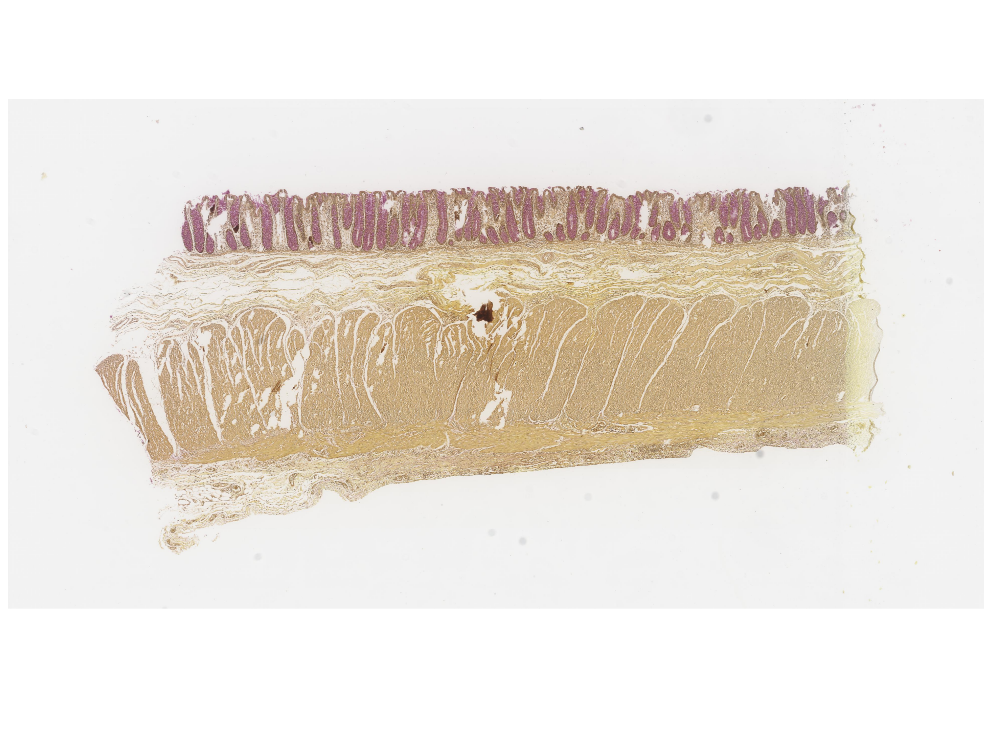
\includegraphics[width=0.25\textwidth,height=\textheight]{./screenshots/mucicarmine_screenshot.png}}
\href{https://images.patolojiatlasi.com/mucin/mucicarmine.html}{Tam
Ekran Görmek İçin Resmi Tıklayın}

\begin{center}\rule{0.5\linewidth}{0.5pt}\end{center}

\hypertarget{sec-chromogenic-in-situ-hybridization-cish}{%
\section{Chromogenic in situ hybridization
(CISH)}\label{sec-chromogenic-in-situ-hybridization-cish}}

\textbf{Chromogenic in situ hybridization (CISH)}

\href{https://images.patolojiatlasi.com/her2-cish/cish.html}{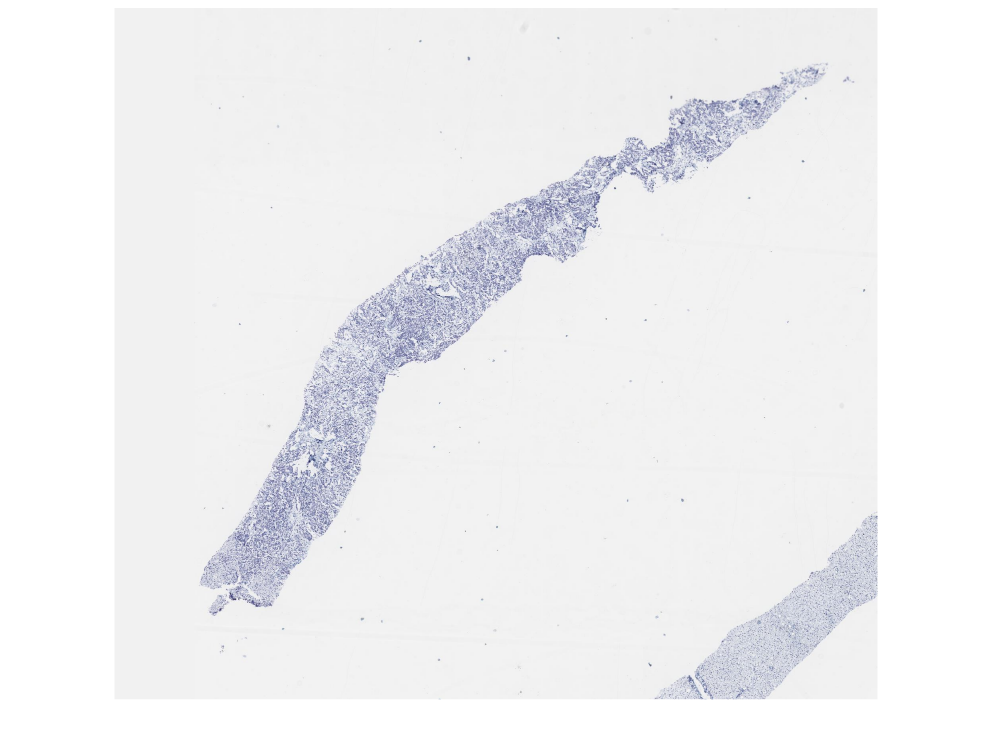
\includegraphics[width=0.25\textwidth,height=\textheight]{./screenshots/cish_screenshot.png}}
\href{https://images.patolojiatlasi.com/her2-cish/cish.html}{Tam Ekran
Görmek İçin Resmi Tıklayın}

\hypertarget{sec-hucre-ici-birikimler}{%
\chapter{Hücre İçi Birikimler}\label{sec-hucre-ici-birikimler}}

\hypertarget{sec-kolesterol-polibi}{%
\section{Kolesterol Polibi}\label{sec-kolesterol-polibi}}

\textbf{Kolesterol Polibi}

\href{https://images.patolojiatlasi.com/cholesterolpolyp/HE.html}{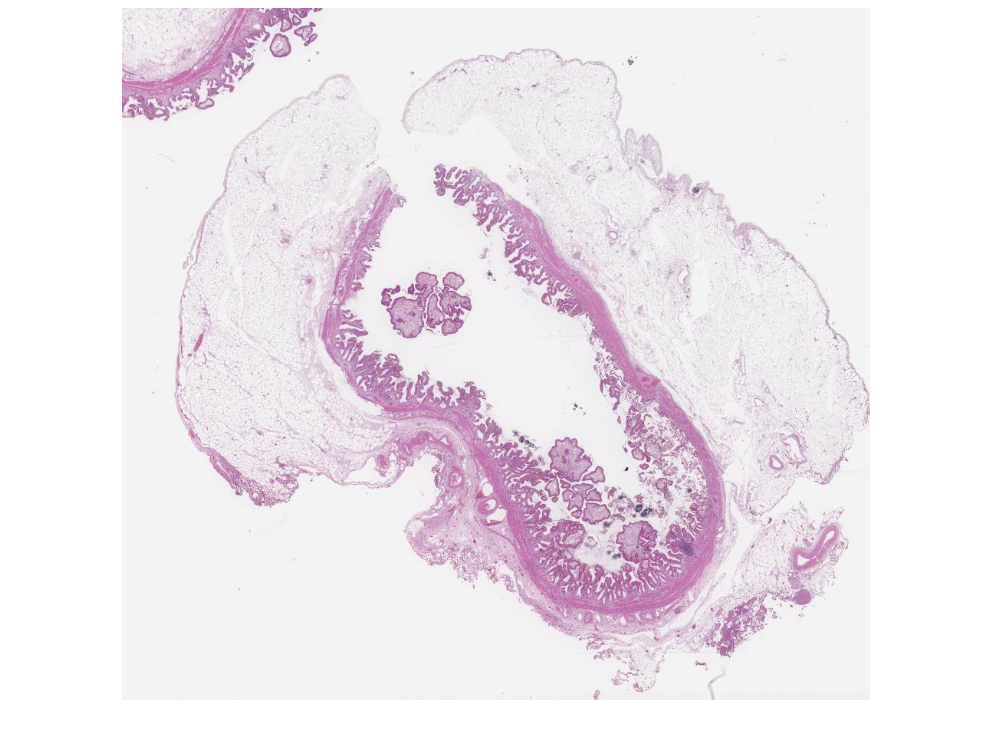
\includegraphics[width=0.25\textwidth,height=\textheight]{./screenshots/cholesterolpolyp_screenshot.png}}
\href{https://images.patolojiatlasi.com/cholesterolpolyp/HE.html}{Tam
Ekran Görmek İçin Resmi Tıklayın}

\hypertarget{sec-glikojen-depo-hastaligi}{%
\section{Glikojen Depo Hastalığı}\label{sec-glikojen-depo-hastaligi}}

\textbf{Karaciğer İğnde Biyopsisinde glikojen depo hastalığı}

\textbf{Hematoksilen Eozin}

\href{https://images.patolojiatlasi.com/glycogenstorage/HE.html}{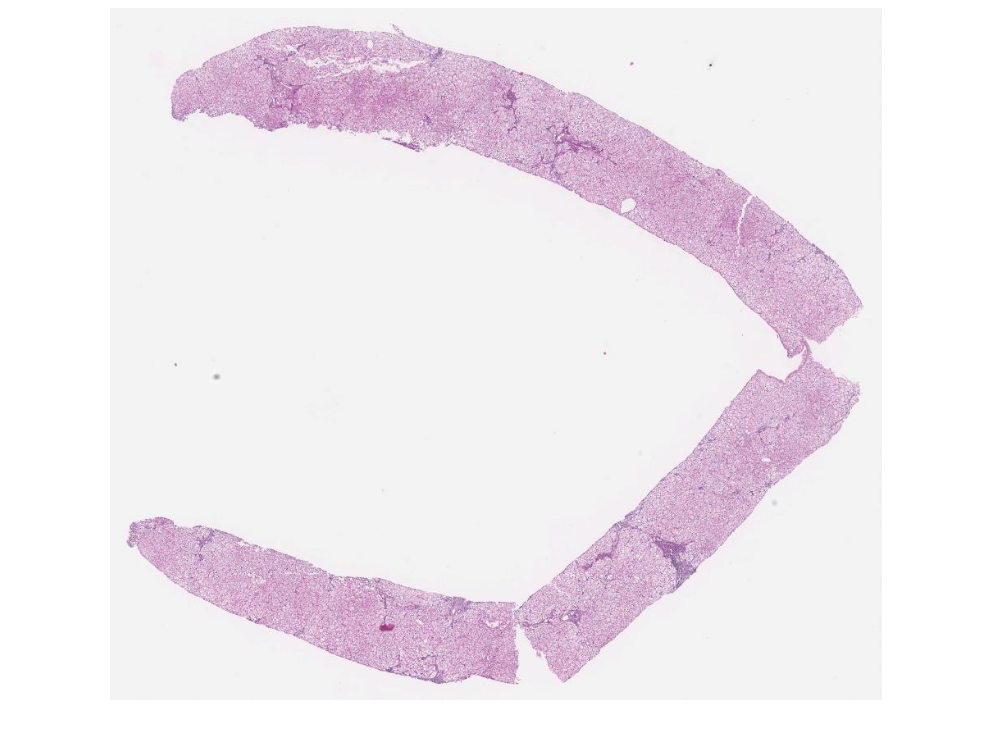
\includegraphics[width=0.25\textwidth,height=\textheight]{./screenshots/glycogenstorage-HE_screenshot.png}}
\href{https://images.patolojiatlasi.com/glycogenstorage/HE.html}{Tam
Ekran Görmek İçin Resmi Tıklayın}

\textbf{PAS}

\href{https://images.patolojiatlasi.com/glycogenstorage/PAS.html}{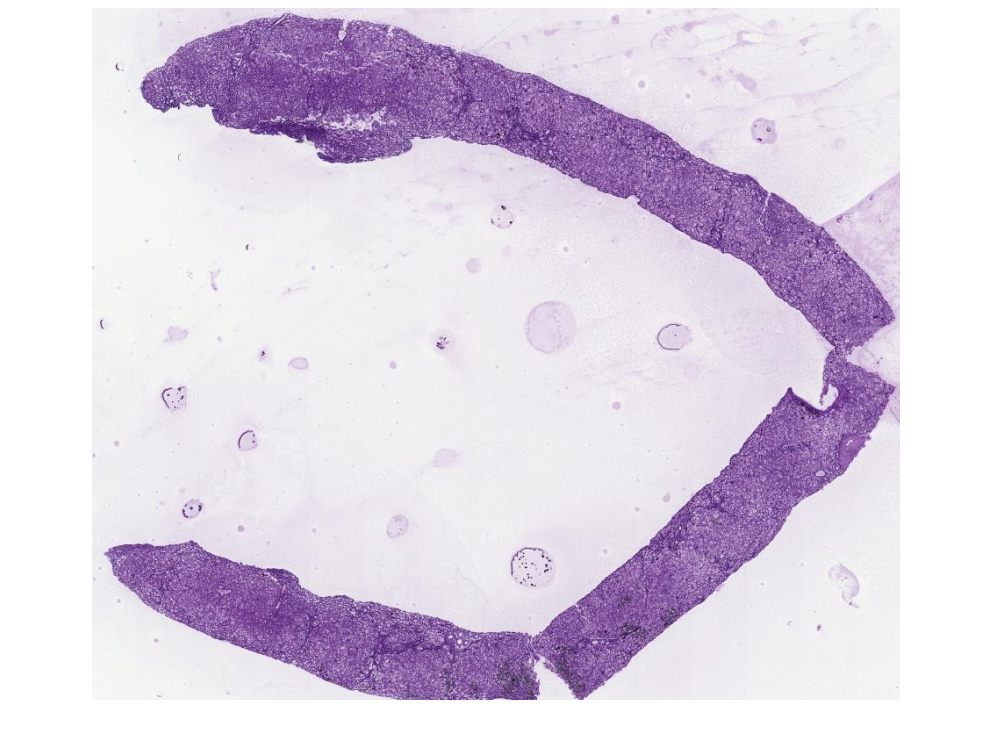
\includegraphics[width=0.25\textwidth,height=\textheight]{./screenshots/glycogenstorage-PAS_screenshot.png}}
\href{https://images.patolojiatlasi.com/glycogenstorage/PAS.html}{Tam
Ekran Görmek İçin Resmi Tıklayın}

\textbf{PASD}

\href{https://images.patolojiatlasi.com/glycogenstorage/PASD.html}{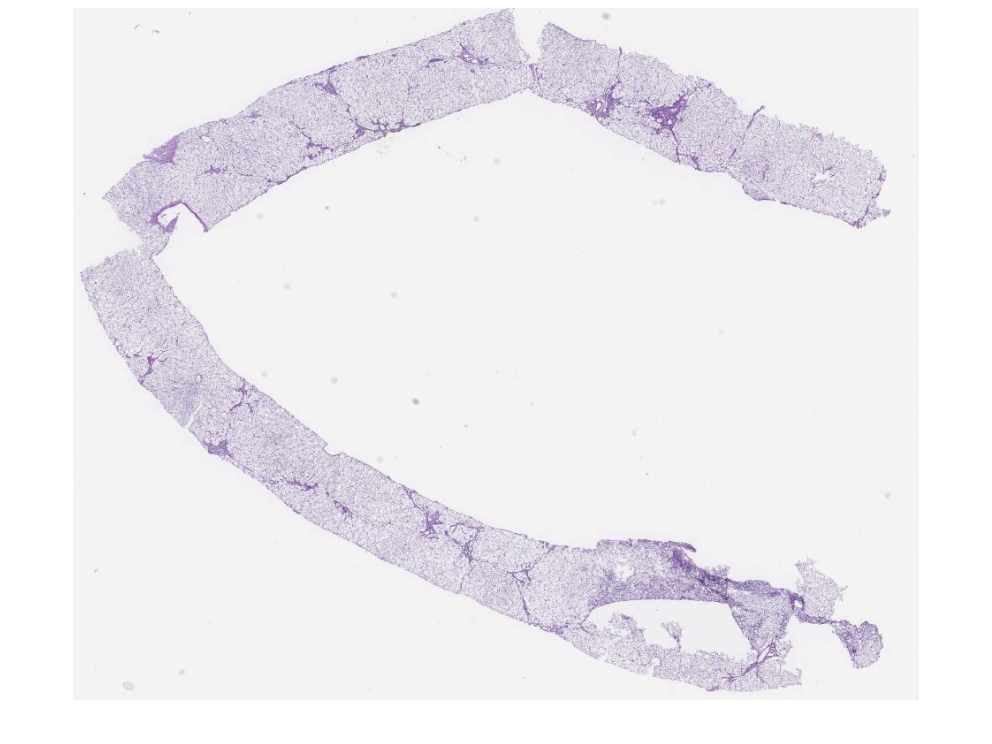
\includegraphics[width=0.25\textwidth,height=\textheight]{./screenshots/glycogenstorage-PASD_screenshot.png}}
\href{https://images.patolojiatlasi.com/glycogenstorage/PASD.html}{Tam
Ekran Görmek İçin Resmi Tıklayın}

\hypertarget{sec-antrakoz-antrakotik-pigment}{%
\section{Antrakoz, Antrakotik
Pigment}\label{sec-antrakoz-antrakotik-pigment}}

Torakal bölge lenf nodunda antrakotik pigment

\href{https://images.patolojiatlasi.com/template/HE.html}{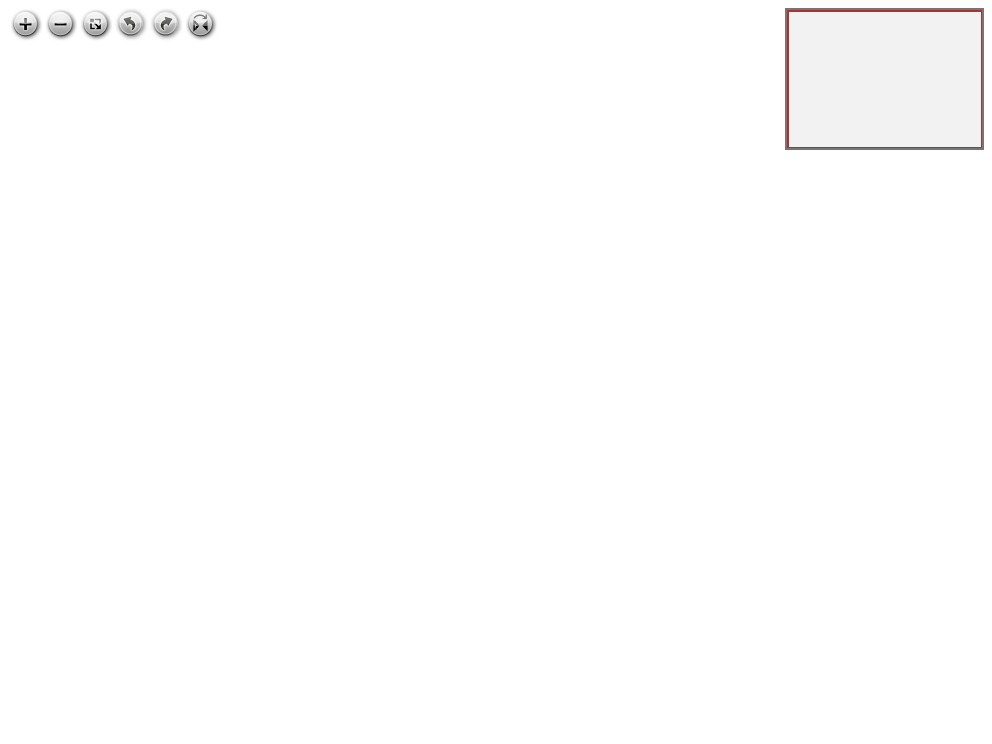
\includegraphics[width=0.25\textwidth,height=\textheight]{./screenshots/template_screenshot.png}}
\href{https://images.patolojiatlasi.com/anthracosis/HE.html}{Click for
Full Screen WSI}

\href{https://images.patolojiatlasi.com/template/HE.html}{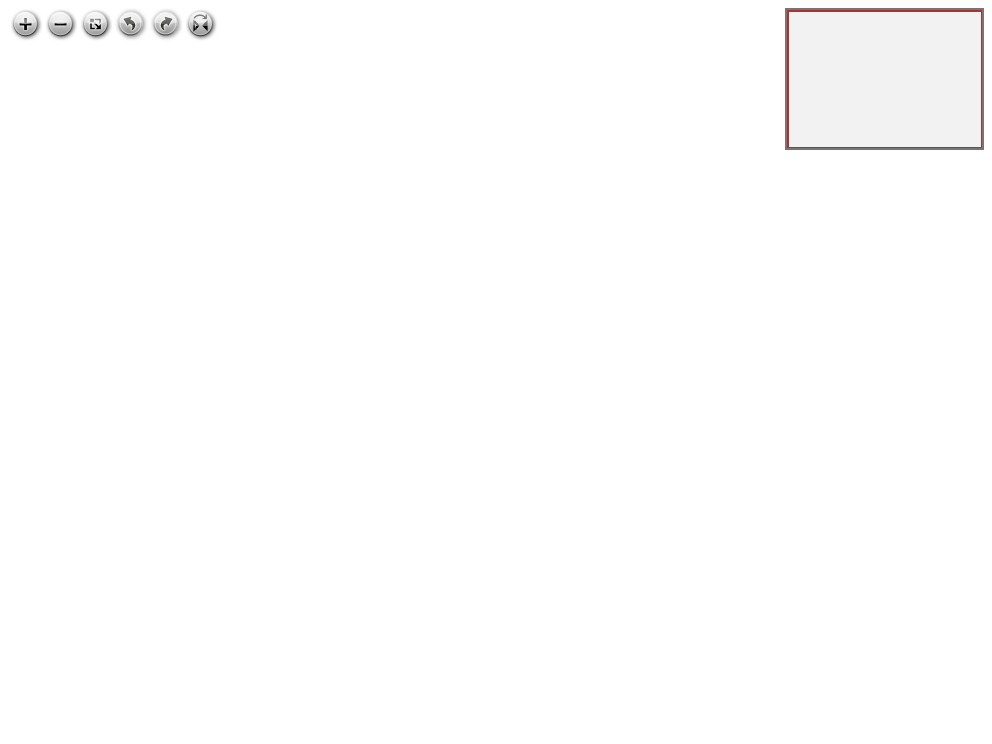
\includegraphics[width=0.25\textwidth,height=\textheight]{./screenshots/template_screenshot.png}}
\href{https://images.patolojiatlasi.com/anthracosis/HE2.html}{Click for
Full Screen WSI}

\hypertarget{sec-melanosis-coli}{%
\section{Melanosis Coli}\label{sec-melanosis-coli}}

\textbf{Melanozis Koli}

\href{https://images.patolojiatlasi.com/template/HE.html}{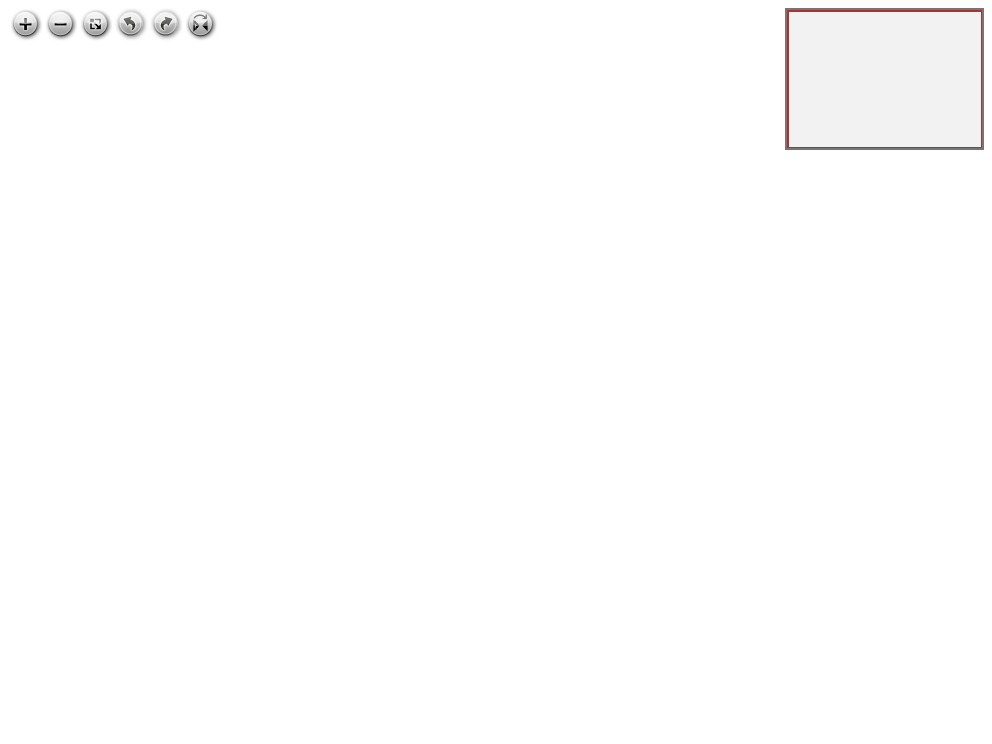
\includegraphics[width=0.25\textwidth,height=\textheight]{./screenshots/template_screenshot.png}}
\href{https://images.patolojiatlasi.com/melanosiscoli/HE.html}{Tam Ekran
Görmek İçin Resmi Tıklayın}

\textbf{Melanozis Koli PAS}

\href{https://images.patolojiatlasi.com/template/HE.html}{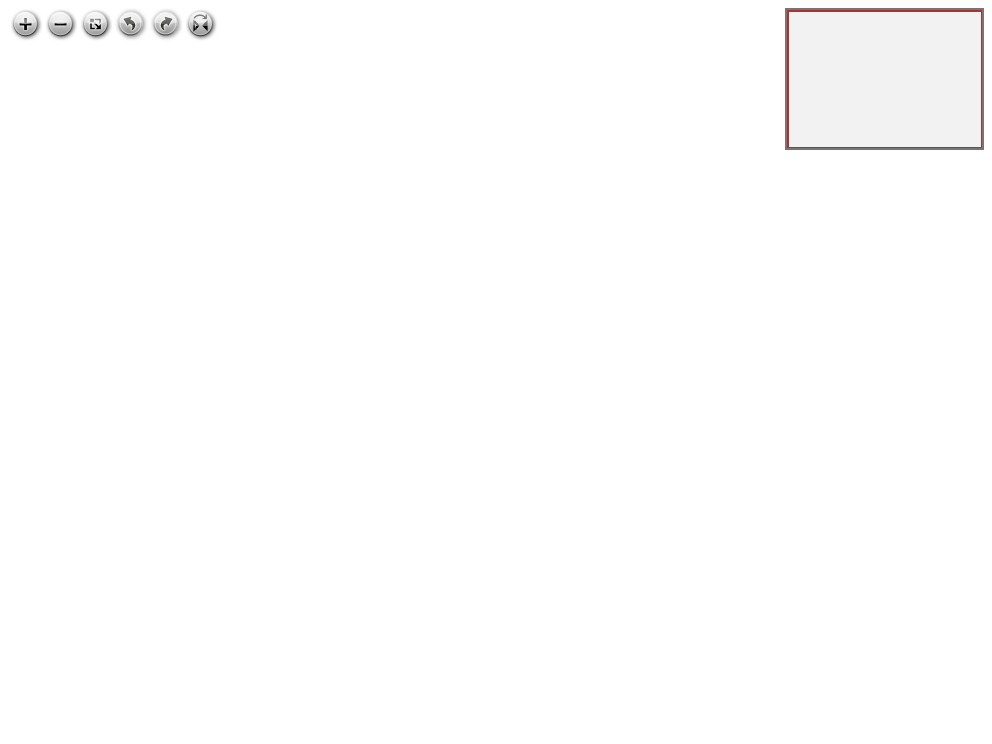
\includegraphics[width=0.25\textwidth,height=\textheight]{./screenshots/template_screenshot.png}}
\href{https://images.patolojiatlasi.com/melanosiscoli/PAS.html}{Tam
Ekran Görmek İçin Resmi Tıklayın}

\hypertarget{sec-hucre-disi-birikimler}{%
\chapter{Hücre Dışı Birikimler}\label{sec-hucre-disi-birikimler}}

\hypertarget{sec-okronozis}{%
\section{Okronozis}\label{sec-okronozis}}

\textbf{Okronozis}

\href{https://images.patolojiatlasi.com/template/HE.html}{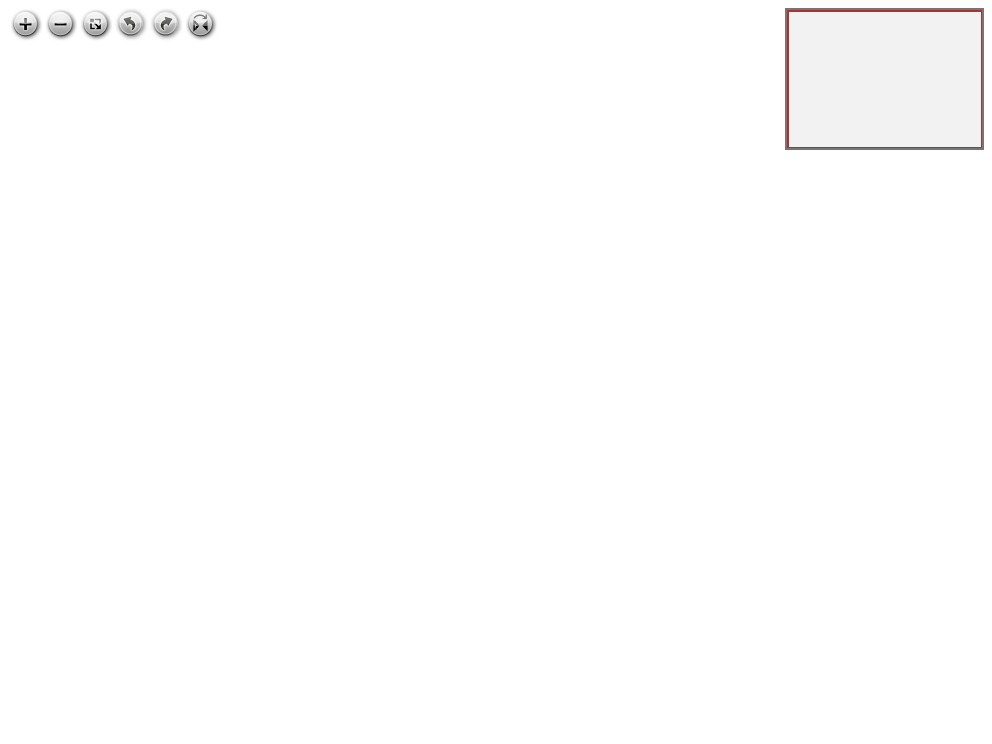
\includegraphics[width=0.25\textwidth,height=\textheight]{./screenshots/template_screenshot.png}}
\href{https://images.patolojiatlasi.com/ochronosis/HE.html}{Tam Ekran
Görmek İçin Resmi Tıklayın}

\hypertarget{sec-hucre-hasari}{%
\chapter{Hücre Hasarı}\label{sec-hucre-hasari}}

\hypertarget{sec-reaktif-atipi}{%
\section{Reaktif Atipi, ülsere kolon polibi}\label{sec-reaktif-atipi}}

\textbf{Reaktif Atipi, ülsere kolon polibi}

\href{https://images.patolojiatlasi.com/template/HE.html}{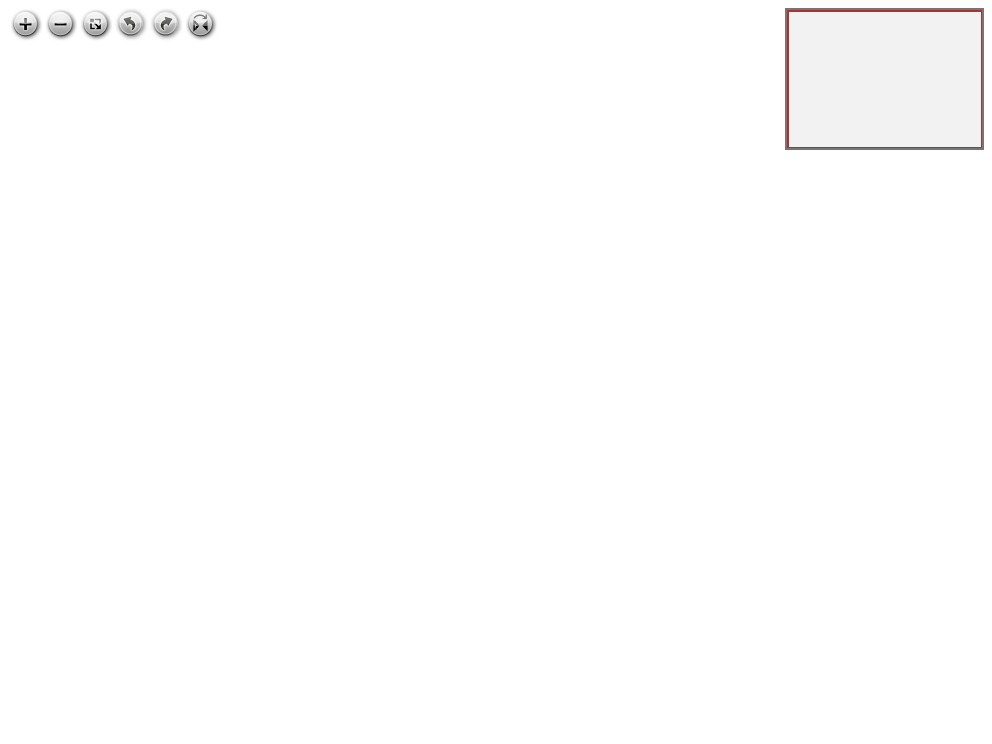
\includegraphics[width=0.25\textwidth,height=\textheight]{./screenshots/template_screenshot.png}}
\href{https://images.patolojiatlasi.com/reactive-atypia/HE.html}{Tam
Ekran Görmek İçin Resmi Tıklayın}

\hypertarget{sec-hemodinamik-bozukluklar}{%
\chapter{Hemodinamik Bozukluklar}\label{sec-hemodinamik-bozukluklar}}

\hypertarget{sec-iskemi-ve-nekroz}{%
\section{İskemi ve Nekroz}\label{sec-iskemi-ve-nekroz}}

\hypertarget{sec-yag-nekrozu-sabunlasma}{%
\subsection{Yağ nekrozu ve
Sabunlaşma}\label{sec-yag-nekrozu-sabunlasma}}

\textbf{Yağ dokuda yağ nekrozu ve sabunlaşma}

\href{https://images.patolojiatlasi.com/template/HE.html}{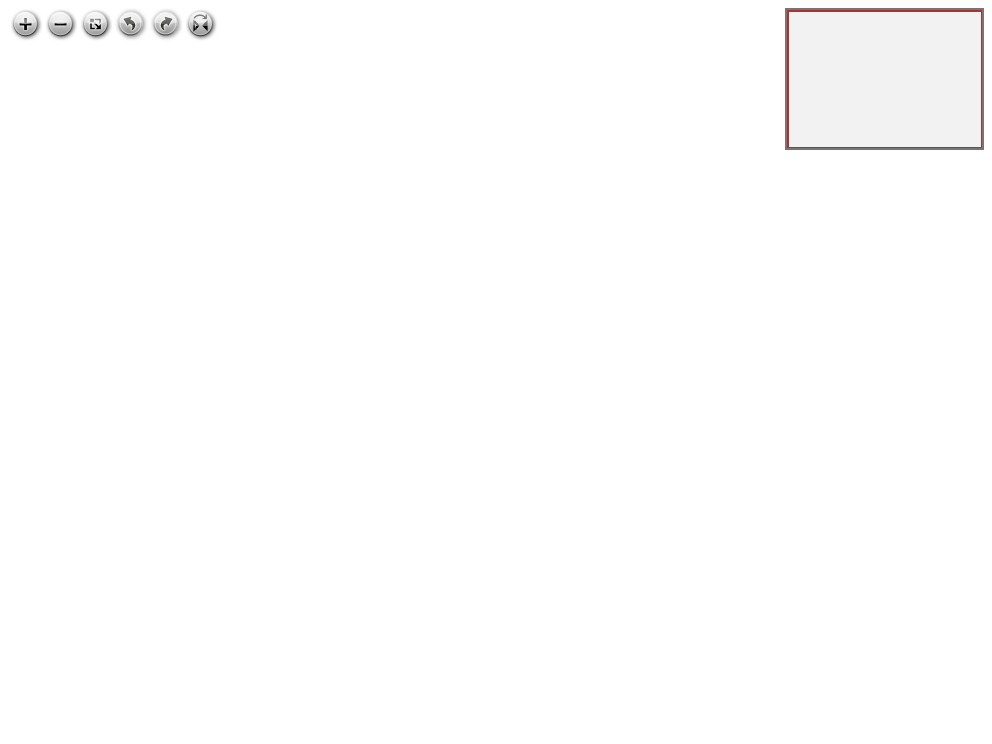
\includegraphics[width=0.25\textwidth,height=\textheight]{./screenshots/template_screenshot.png}}
\href{https://images.patolojiatlasi.com/fat-necrosis/HE.html}{Tam Ekran
Görmek İçin Resmi Tıklayın}

\hypertarget{sec-amiloidoz}{%
\chapter{Amiloidoz (Amiloid Birikimi)}\label{sec-amiloidoz}}

\hypertarget{sec-amiloidoz-kristal-viyole}{%
\section{Kristal Viyole}\label{sec-amiloidoz-kristal-viyole}}

\textbf{Damar duvarlarında amiloid birikimi}

\href{https://images.patolojiatlasi.com/amyloid/crystalviolet.html}{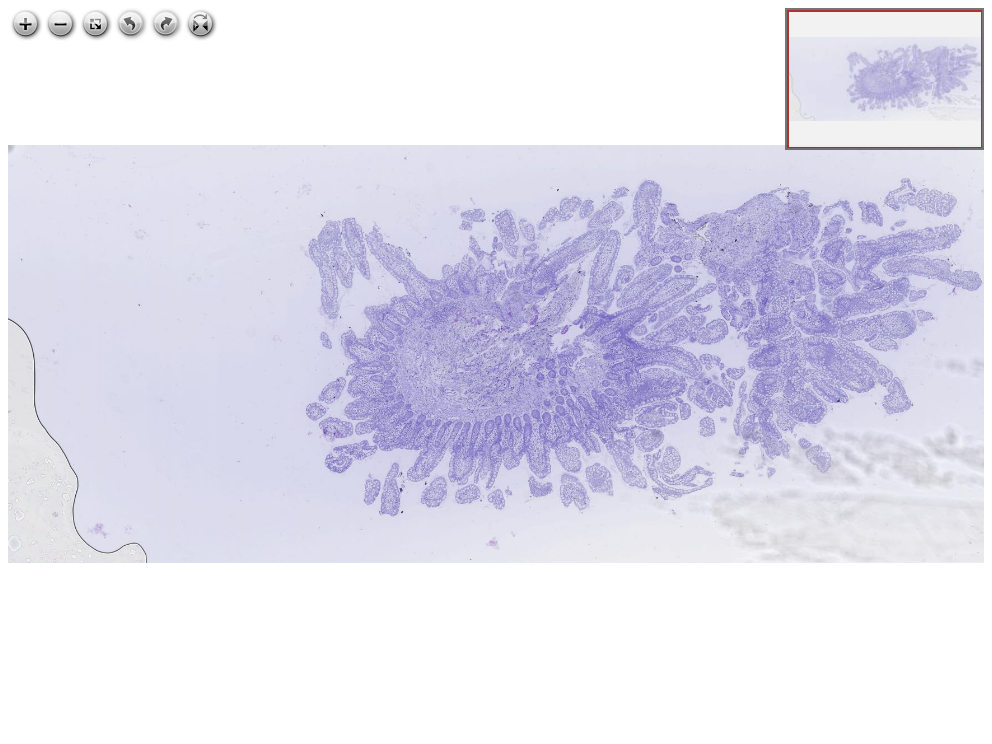
\includegraphics[width=0.25\textwidth,height=\textheight]{./screenshots/crystalviolet_screenshot.png}}
\href{https://images.patolojiatlasi.com/amyloid/crystalviolet.html}{Tam
Ekran Görmek İçin Resmi Tıklayın}

\hypertarget{sec-amiloidoz-kongo-kirmizisi}{%
\section{Kongo Kırmızısı}\label{sec-amiloidoz-kongo-kirmizisi}}

\hypertarget{sec-amiloidoz-kongo-kirmizisi-cift-kiricilik}{%
\section{Kongo Kırmızısı Çift
Kırıcılık}\label{sec-amiloidoz-kongo-kirmizisi-cift-kiricilik}}

\url{https://www.youtube.com/watch?v=U9glkfQLTm4}

\hypertarget{sec-tamir-mekanizmalari}{%
\chapter{Tamir Mekanizmaları}\label{sec-tamir-mekanizmalari}}

Bu sayfadaki görüntülere artırılmış gerçeklik (augmented reality) ile de
ulaşabilirsiniz\footnote{\href{https://github.com/veterinarypathology3d}{Tarık
  Atmaca} tarafından \url{https://veterinarypathology3d.com/}
  geliştirilmiştir.}.

Karekodu cep telefonunuza okutun:

\begin{figure}


\includegraphics[width=1.04167in,height=\textheight]{images/AR-tamir.jpeg} \hfill{}

\end{figure}

Link ile açılan sayfaya ve kamera erişimine izin verin. Sonra kamerayı
bu sayfadaki patoloji resimlerine tutun. Tanılar cep telefonunuzda
görünecektir.

\url{https://www.youtube.com/watch?v=76bOJIiT29Y}

\hypertarget{sec-fibrozis}{%
\section{Fibrozis}\label{sec-fibrozis}}

Kolesistit spesmeninde gelişmekte olan genç fibrozis

\href{https://images.patolojiatlasi.com/fibrosis/HE.html}{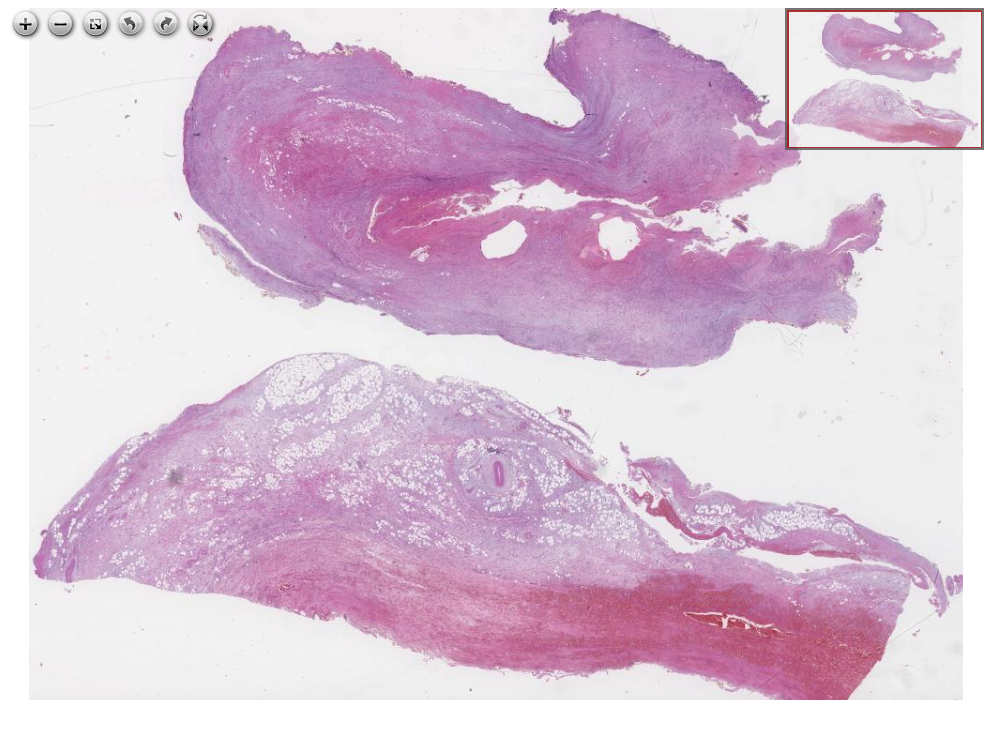
\includegraphics[width=0.25\textwidth,height=\textheight]{./screenshots/fibrosis_screenshot.png}}
\href{https://images.patolojiatlasi.com/fibrosis/HE.html}{Tam Ekran
Görmek İçin Resmi Tıklayın}

\hypertarget{sec-keloid-skar}{%
\section{Keloid - Skar}\label{sec-keloid-skar}}

Keloid Skar oluşumu

\href{https://images.patolojiatlasi.com/keloid-scar/HE.html}{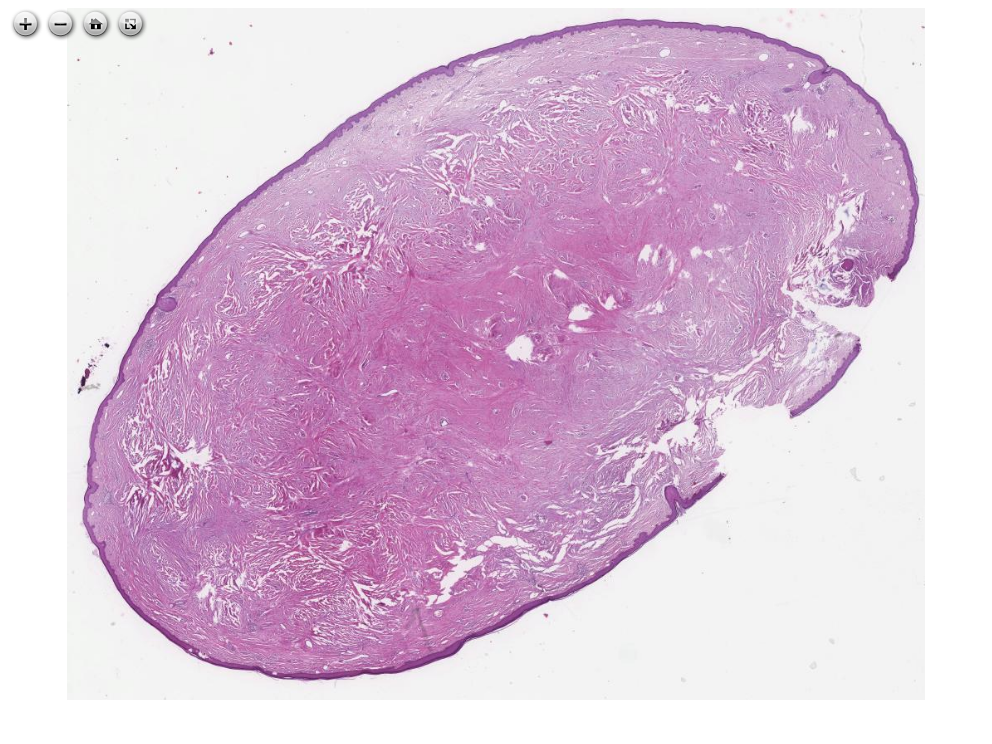
\includegraphics[width=0.25\textwidth,height=\textheight]{./screenshots/keloid-scar_screenshot.png}}
\href{https://images.patolojiatlasi.com/keloid-scar/HE.html}{Tam Ekran
Görmek İçin Resmi Tıklayın}

\hypertarget{sec-erozyon}{%
\chapter{Erozyon}\label{sec-erozyon}}

\hypertarget{sec-mide-mukozasinda-erozyon}{%
\section{Mide mukozasında erozyon}\label{sec-mide-mukozasinda-erozyon}}

\textbf{Mide mukozasında erozyon}

\href{https://images.patolojiatlasi.com/erosion/HE.html}{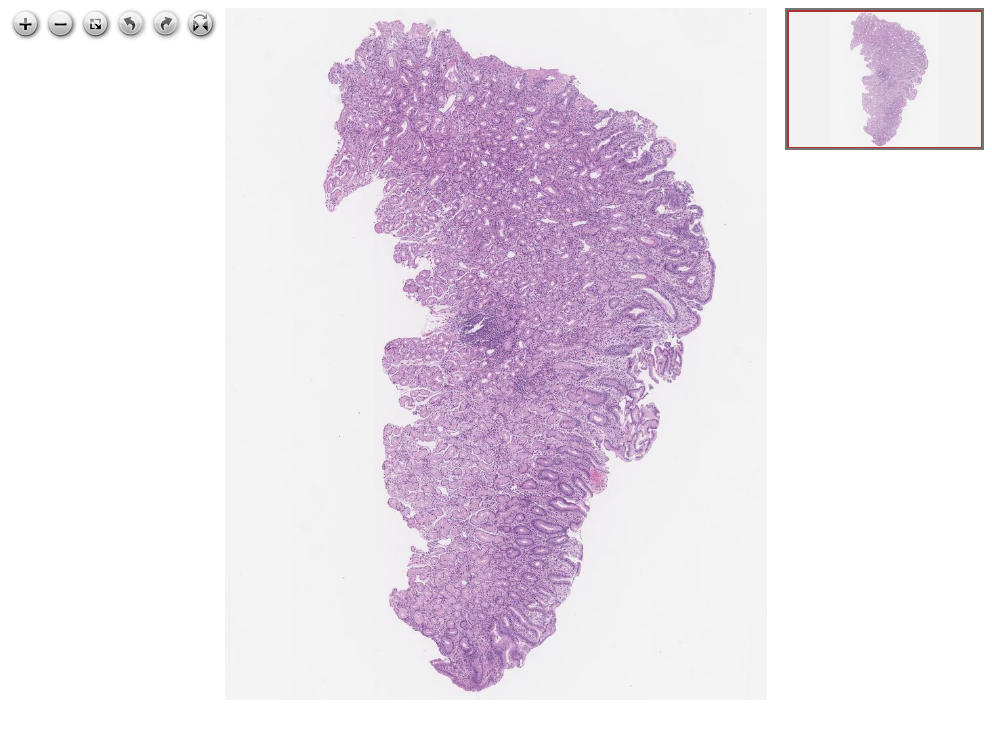
\includegraphics[width=0.25\textwidth,height=\textheight]{./screenshots/erosion_screenshot.png}}
\href{https://images.patolojiatlasi.com/erosion/HE.html}{Tam Ekran
Görmek İçin Resmi Tıklayın}

\part{İnflamasyon}

\hypertarget{sec-akut-inflamasyon}{%
\chapter{Akut İnflamasyon}\label{sec-akut-inflamasyon}}

\hypertarget{sec-akut-appendisit}{%
\section{Akut Appendisit}\label{sec-akut-appendisit}}

\textbf{Akut appendisit}

\href{https://images.patolojiatlasi.com/acute-appendicitis/HE.html}{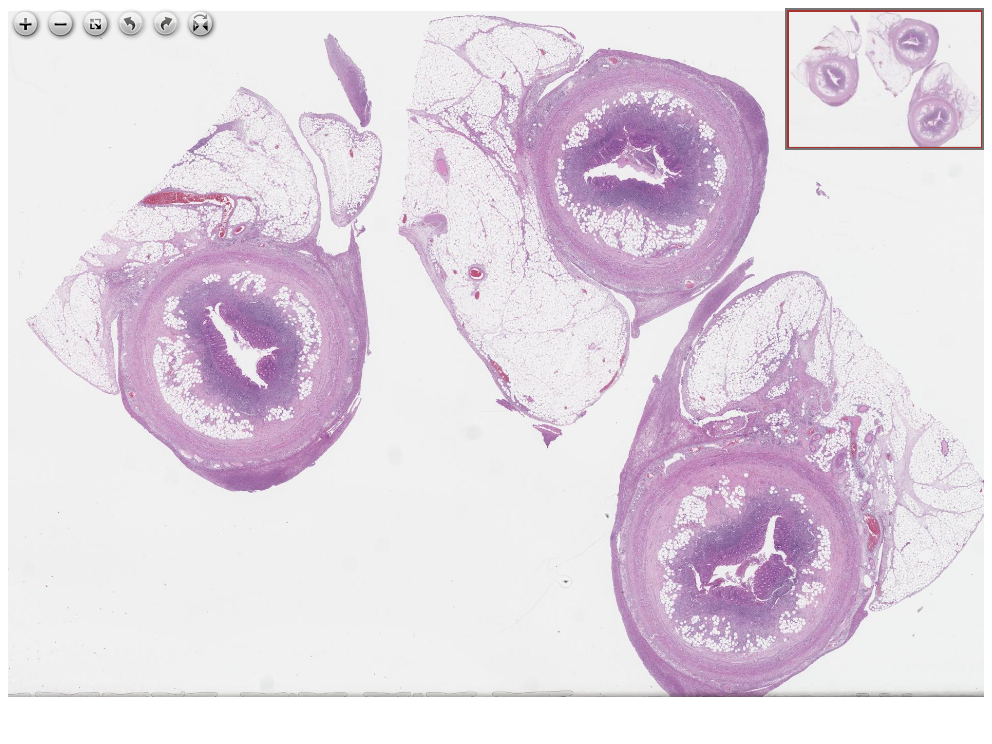
\includegraphics[width=0.25\textwidth,height=\textheight]{./screenshots/acute-appendicitis_screenshot.png}}
\href{https://images.patolojiatlasi.com/acute-appendicitis/HE.html}{Tam
Ekran Görmek İçin Resmi Tıklayın}

\hypertarget{sec-kronik-inflamasyon}{%
\chapter{Kronik İnflamasyon}\label{sec-kronik-inflamasyon}}

\hypertarget{sec-hidronefroz-kronik-pyelonefrit}{%
\section{Hidronefroz ve Kronik
Pyelonefrit}\label{sec-hidronefroz-kronik-pyelonefrit}}

\textbf{Hidronefroz ve Kronik Pyelonefrit}

\href{https://images.patolojiatlasi.com/template/HE.html}{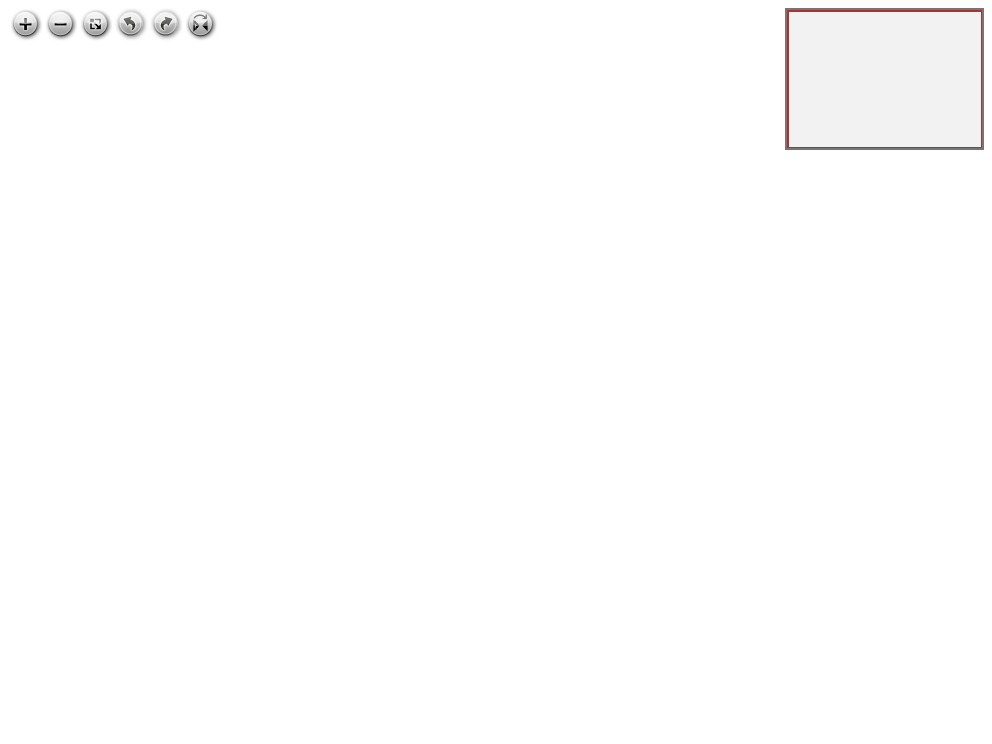
\includegraphics[width=0.25\textwidth,height=\textheight]{./screenshots/template_screenshot.png}}
\href{https://images.patolojiatlasi.com/chronicpyelonephritis/HE1.html}{Tam
Ekran Görmek İçin Resmi Tıklayın}

\hypertarget{sec-kronik-pyelonefrit}{%
\section{Kronik Pyelonefrit}\label{sec-kronik-pyelonefrit}}

\textbf{Kronik Pyelonefrit}

\href{https://images.patolojiatlasi.com/template/HE.html}{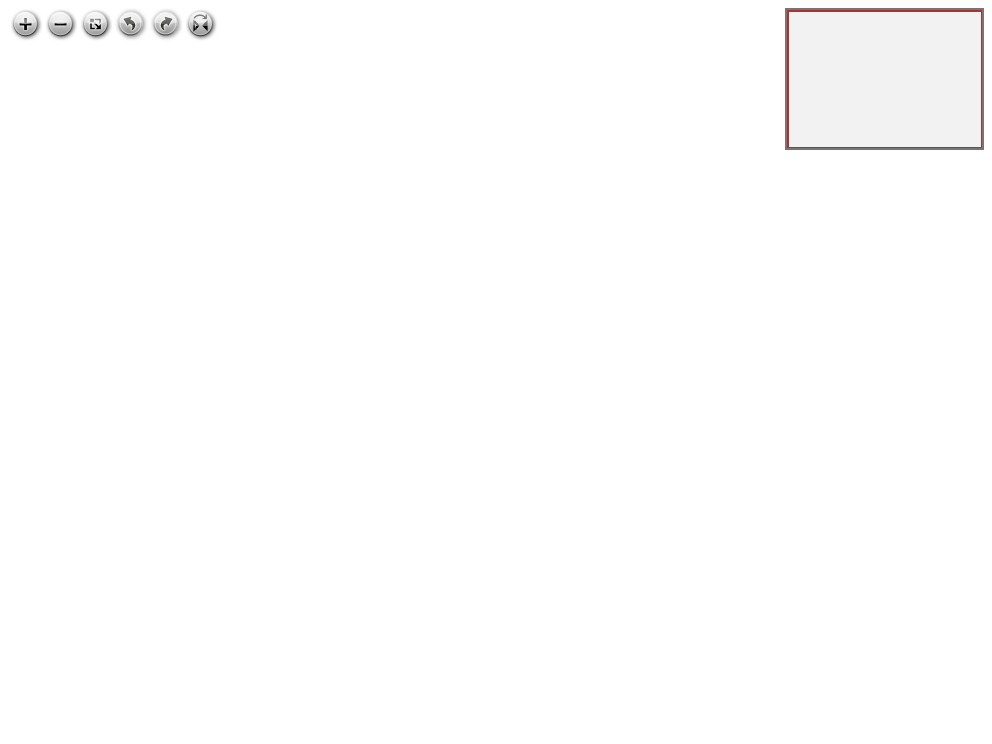
\includegraphics[width=0.25\textwidth,height=\textheight]{./screenshots/template_screenshot.png}}
\href{https://images.patolojiatlasi.com/chronic-pyelonephritis/HE.html}{Tam
Ekran Görmek İçin Resmi Tıklayın}

\hypertarget{sec-granulamatoz-inflamasyon}{%
\chapter{Granülamatöz İnflamasyon}\label{sec-granulamatoz-inflamasyon}}

\hypertarget{sec-nekrotizan-granulamatoz-inflamasyon}{%
\section{Nekrotizan Granülamatöz
İnflamasyon}\label{sec-nekrotizan-granulamatoz-inflamasyon}}

\textbf{Karaciğer dokusunda nekrotizan granülamatöz inflamasyon}

\href{https://images.patolojiatlasi.com/necrotisinggranuloma/HE.html}{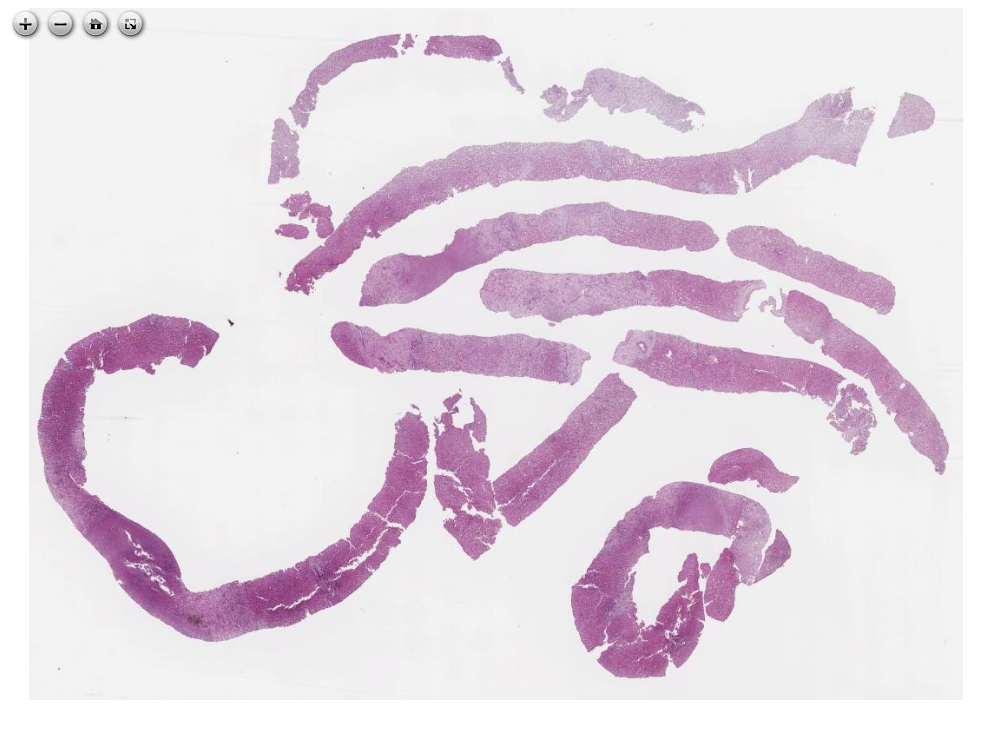
\includegraphics[width=0.25\textwidth,height=\textheight]{./screenshots/necrotisinggranuloma_screenshot.png}}
\href{https://images.patolojiatlasi.com/necrotisinggranuloma/HE.html}{Tam
Ekran Görmek İçin Resmi Tıklayın}

\part{İnfeksiyöz Hastalıkların Patolojisi}

\hypertarget{sec-viruslar}{%
\chapter{Viruslar}\label{sec-viruslar}}

\hypertarget{sec-herpes-simplex-virus}{%
\section{Herpes Simplex Virus (HSV)}\label{sec-herpes-simplex-virus}}

\href{https://images.patolojiatlasi.com/HSV/herpesesophagitis/viewer_z0.html}{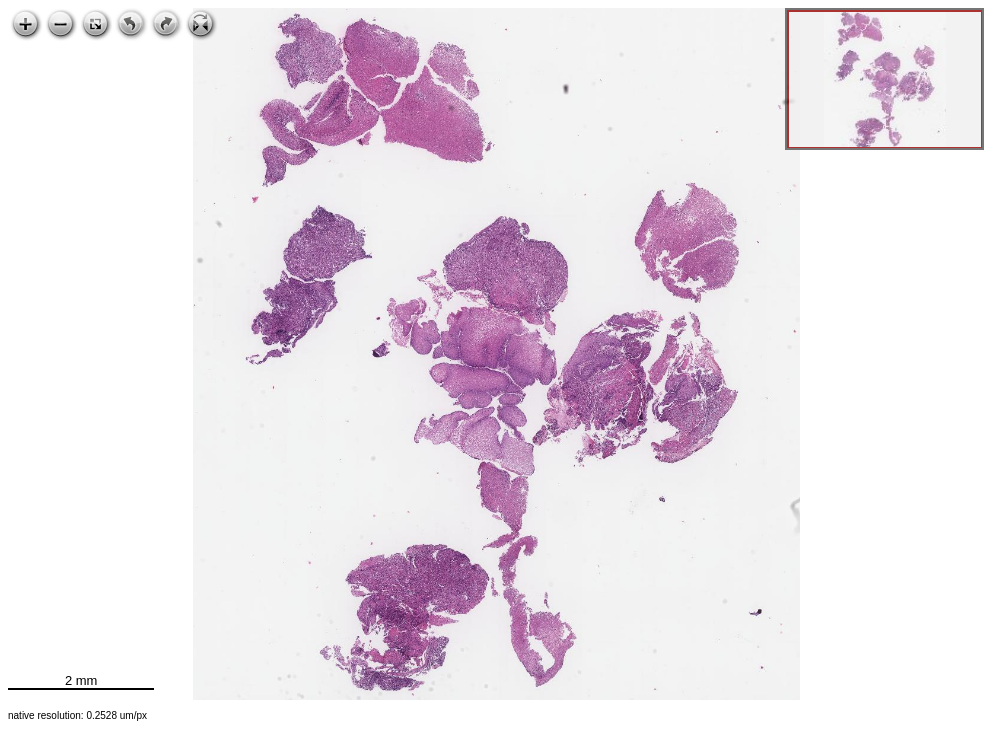
\includegraphics[width=0.25\textwidth,height=\textheight]{./screenshots/herpesesophagitis_screenshot.png}}
\href{https://images.patolojiatlasi.com/HSV/herpesesophagitis/viewer_z0.html}{Tam
Ekran Görmek İçin Resmi Tıklayın}

\hypertarget{sec-molluscum-contagiosum}{%
\section{Molluscum contagiosum}\label{sec-molluscum-contagiosum}}

\textbf{Molluscum contagiosum}

\href{https://images.patolojiatlasi.com/molluscum-contagiosum/HE.html}{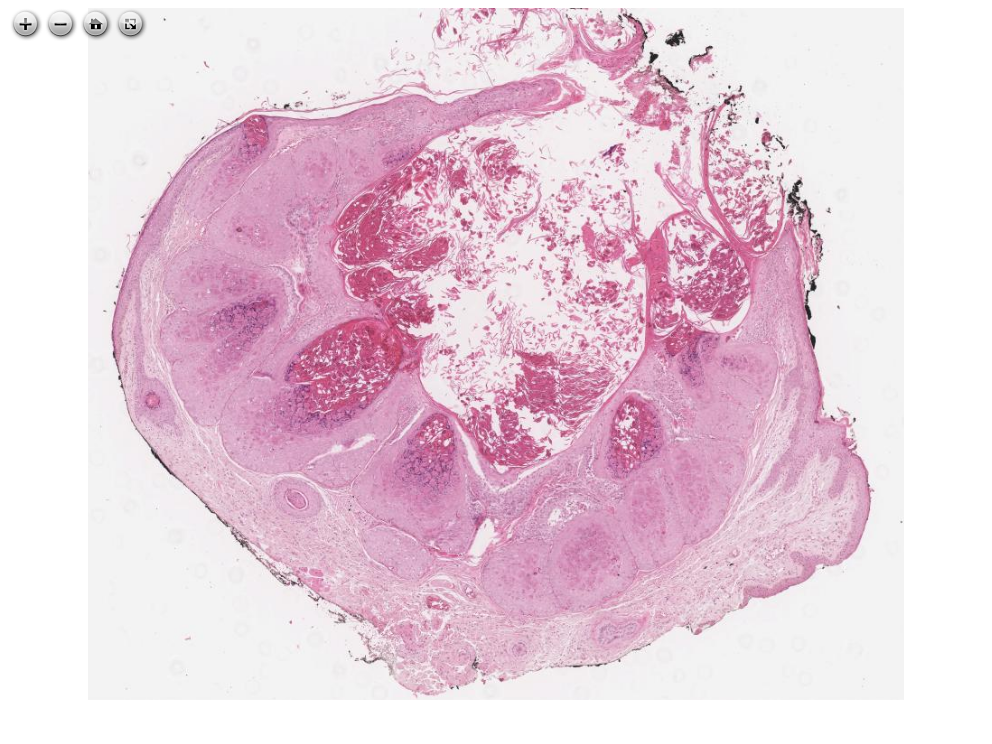
\includegraphics[width=0.25\textwidth,height=\textheight]{./screenshots/molluscum-contagiosum_screenshot.png}}
\href{https://images.patolojiatlasi.com/molluscum-contagiosum/HE.html}{Tam
Ekran Görmek İçin Resmi Tıklayın}

\hypertarget{sec-bakteriler}{%
\chapter{Bakteriler}\label{sec-bakteriler}}

\hypertarget{sec-helicobacter-pylori}{%
\section{Helicobacter pylori}\label{sec-helicobacter-pylori}}

\textbf{Mide'de Helicobacter pylori (H. pylori) HE}

\href{https://images.patolojiatlasi.com/helicobacterpylori/HE.html}{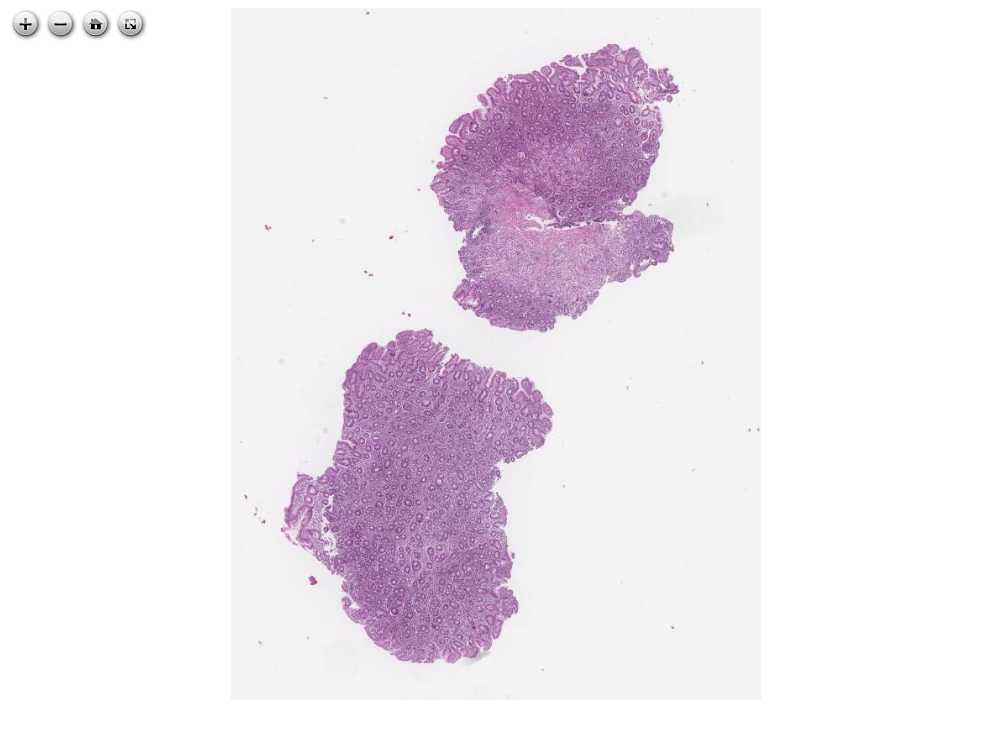
\includegraphics[width=0.25\textwidth,height=\textheight]{./screenshots/helicobacterpylori_screenshot.png}}
\href{https://images.patolojiatlasi.com/helicobacterpylori/HE.html}{Tam
Ekran Görmek İçin Resmi Tıklayın}

\textbf{Mide'de Helicobacter pylori (H. pylori) Warthin Starry
Histokimyası}

\href{https://images.patolojiatlasi.com/helicobacterpylori/warthinstarry.html}{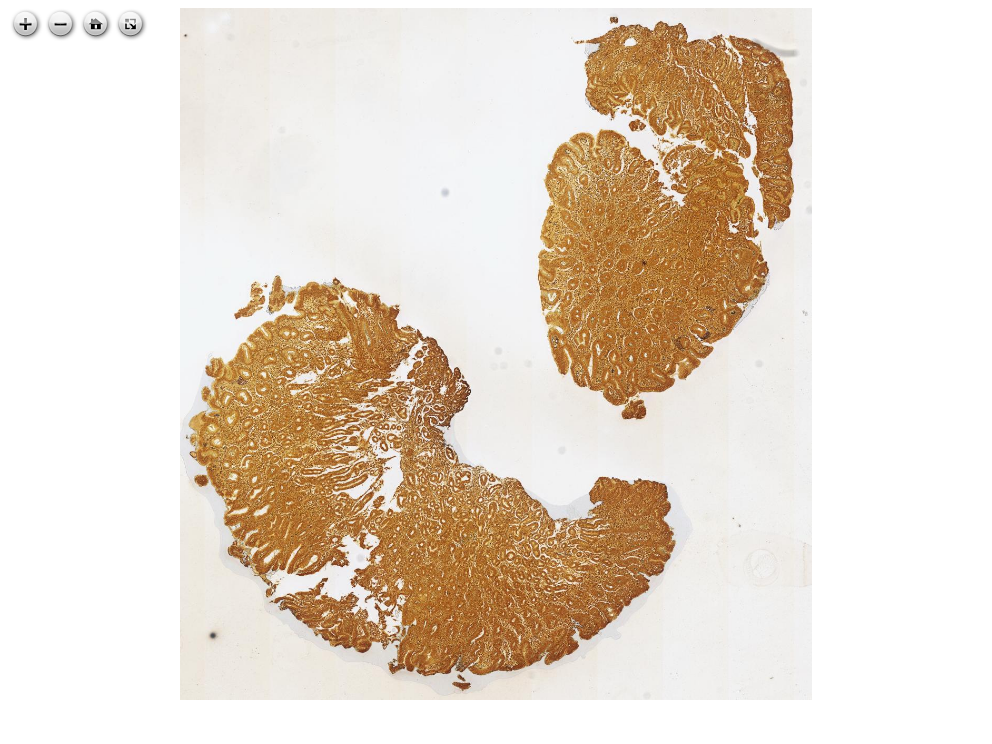
\includegraphics[width=0.25\textwidth,height=\textheight]{./screenshots/helicobacterpyloriWS_screenshot.png}}
\href{https://images.patolojiatlasi.com/helicobacterpylori/warthinstarry.html}{Tam
Ekran Görmek İçin Resmi Tıklayın}

\textbf{Mide'de Helicobacter pylori (H. pylori) Giemsa Histokimyası}

\href{https://images.patolojiatlasi.com/helicobacterpylori/giemsa.html}{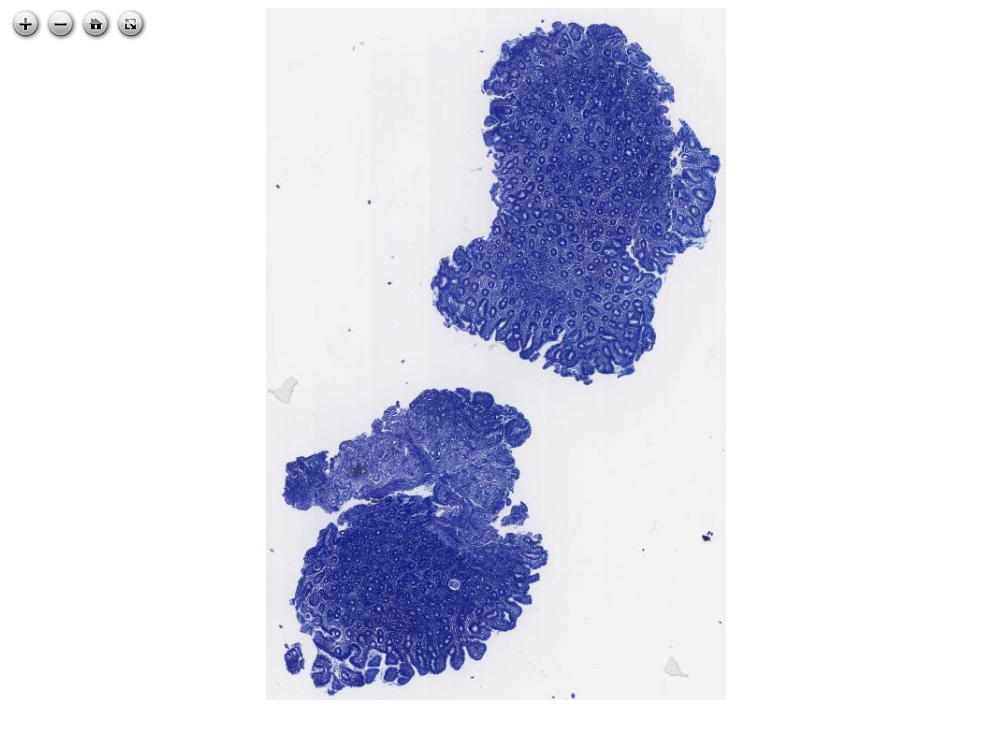
\includegraphics[width=0.25\textwidth,height=\textheight]{./screenshots/helicobacterpyloriGiemsa_screenshot.png}}
\href{https://images.patolojiatlasi.com/helicobacterpylori/giemsa.html}{Tam
Ekran Görmek İçin Resmi Tıklayın}

\textbf{Mide'de Helicobacter pylori (H. pylori) İmmünohistokimyası}

\href{https://images.patolojiatlasi.com/helicobacterpylori/IHC.html}{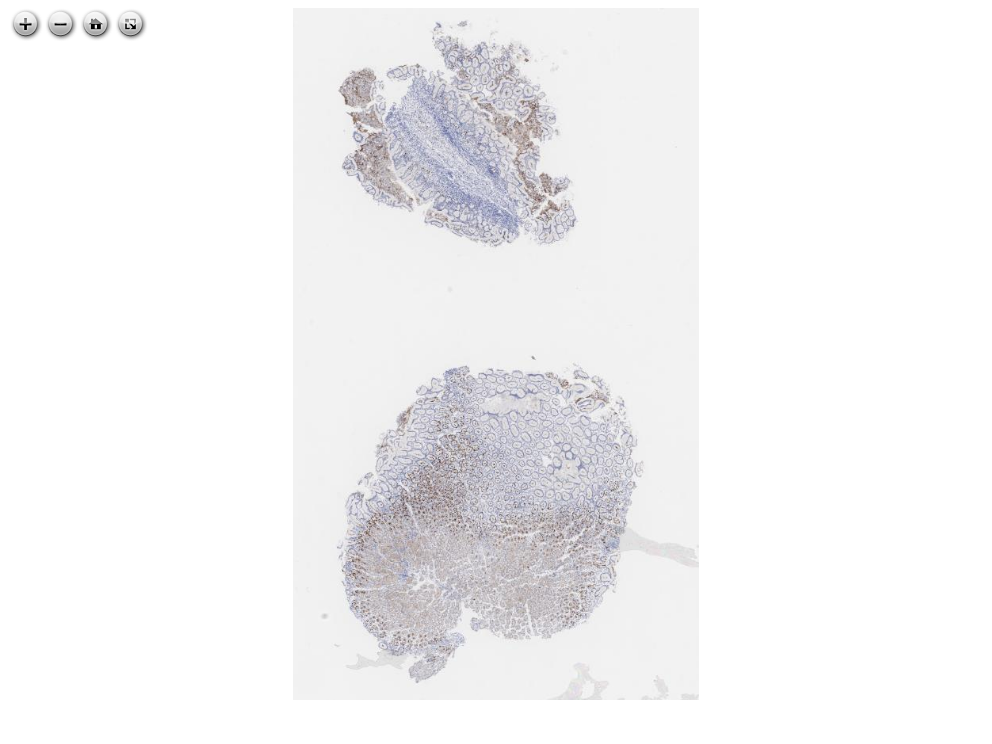
\includegraphics[width=0.25\textwidth,height=\textheight]{./screenshots/helicobacterpyloriIHC_screenshot.png}}
\href{https://images.patolojiatlasi.com/helicobacterpylori/IHC.html}{Tam
Ekran Görmek İçin Resmi Tıklayın}

\hypertarget{sec-mantarlar}{%
\chapter{Mantarlar}\label{sec-mantarlar}}

\hypertarget{sec-candida-albicans-in-cervicovaginal-smear}{%
\section{\texorpdfstring{Candida \emph{albicans} in cervicovaginal
smear}{Candida albicans in cervicovaginal smear}}\label{sec-candida-albicans-in-cervicovaginal-smear}}

\begin{Shaded}
\begin{Highlighting}[]
\FunctionTok{print}\NormalTok{(}\StringTok{"repeating content"}\NormalTok{)}
\end{Highlighting}
\end{Shaded}

\begin{verbatim}
[1] "repeating content"
\end{verbatim}

\href{https://images.patolojiatlasi.com/template/HE.html}{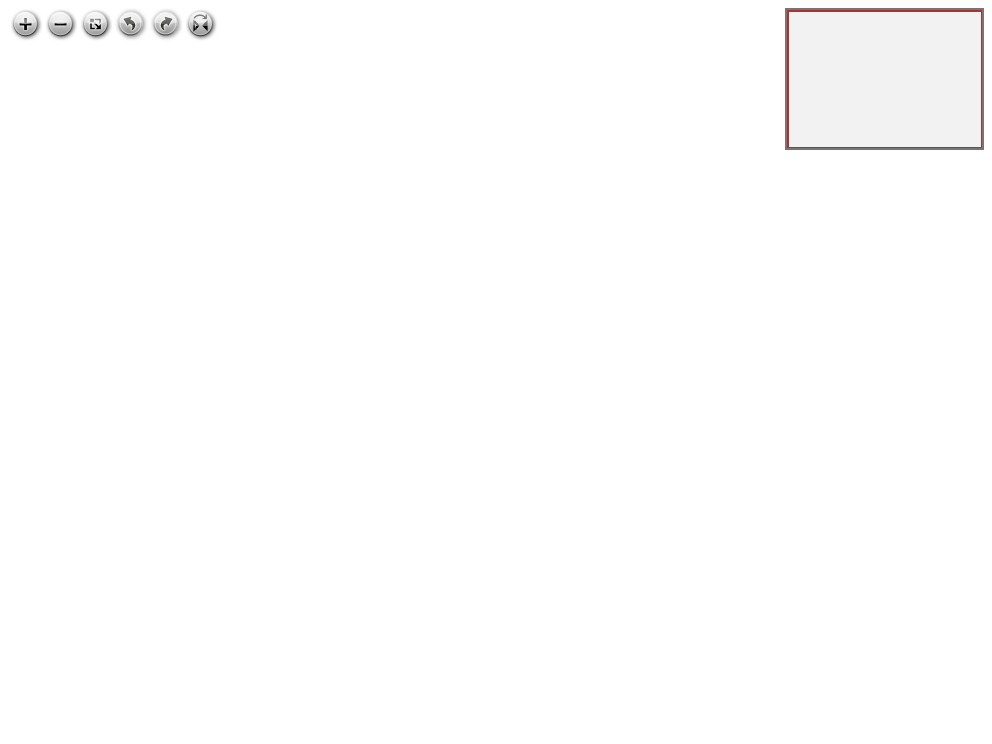
\includegraphics[width=0.25\textwidth,height=\textheight]{./screenshots/template_screenshot.png}}
\href{https://images.patolojiatlasi.com/candidaalbicans/cervicovaginalsmear/viewer_z0.html}{Tam
Ekran Görmek İçin Resmi Tıklayın}

\hypertarget{sec-beyin-mukormikozis}{%
\section{Beyin mukormikozis}\label{sec-beyin-mukormikozis}}

\textbf{Beyin mukormikozis HE}

\href{https://images.patolojiatlasi.com/template/HE.html}{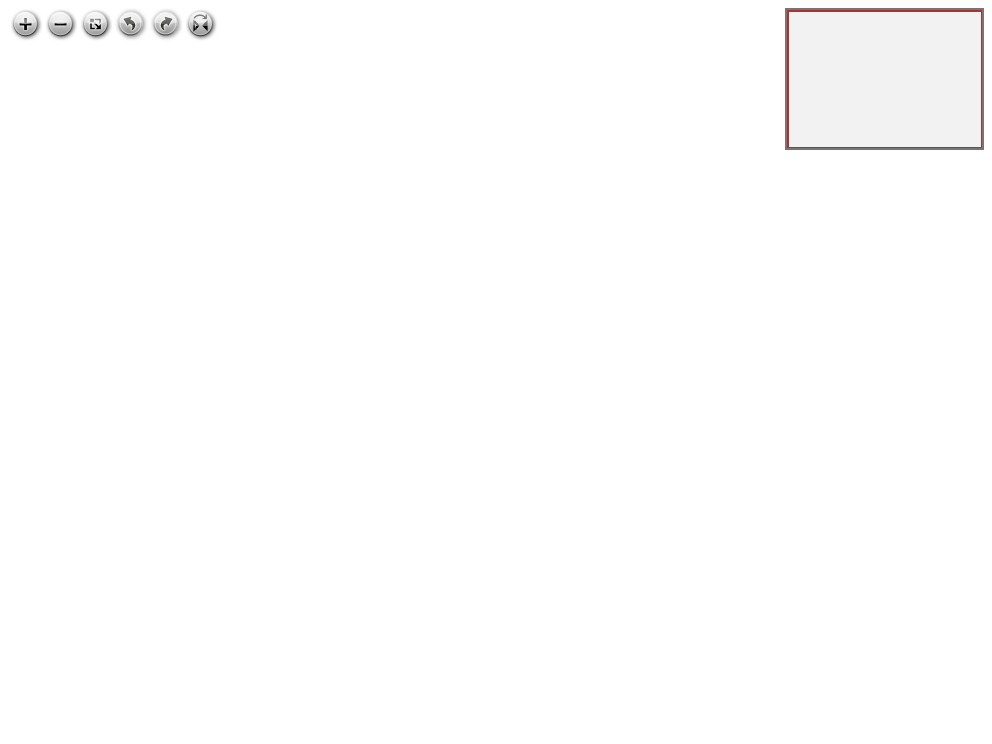
\includegraphics[width=0.25\textwidth,height=\textheight]{./screenshots/template_screenshot.png}}
\href{https://images.patolojiatlasi.com/brain-mucormycosis/HE.html}{Tam
Ekran Görmek İçin Resmi Tıklayın}

\textbf{Beyin mukormikozis GMS}

\href{https://images.patolojiatlasi.com/template/HE.html}{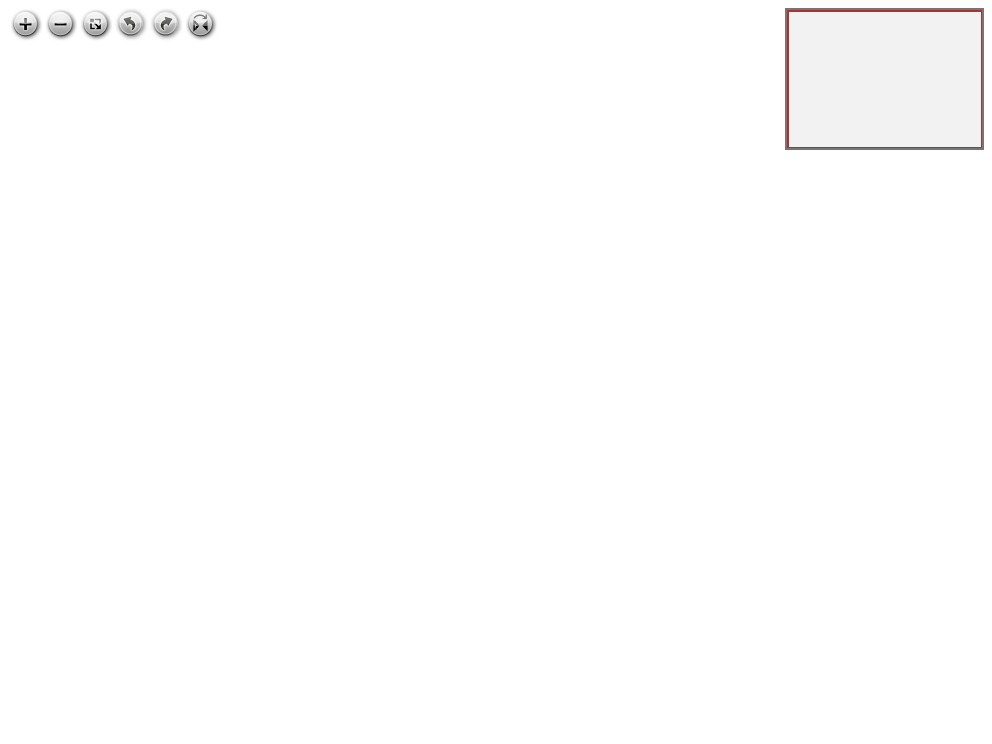
\includegraphics[width=0.25\textwidth,height=\textheight]{./screenshots/template_screenshot.png}}
\href{https://images.patolojiatlasi.com/brain-mucormycosis/HE.html}{Tam
Ekran Görmek İçin Resmi Tıklayın}

\hypertarget{sec-parazitler}{%
\chapter{Parazitler}\label{sec-parazitler}}

\hypertarget{sec-enterobius-vermicularis}{%
\section{Enterobius vermicularis}\label{sec-enterobius-vermicularis}}

\textbf{Enterobius vermicularis}

\href{https://images.patolojiatlasi.com/enterobius-vermicularis/HE.html}{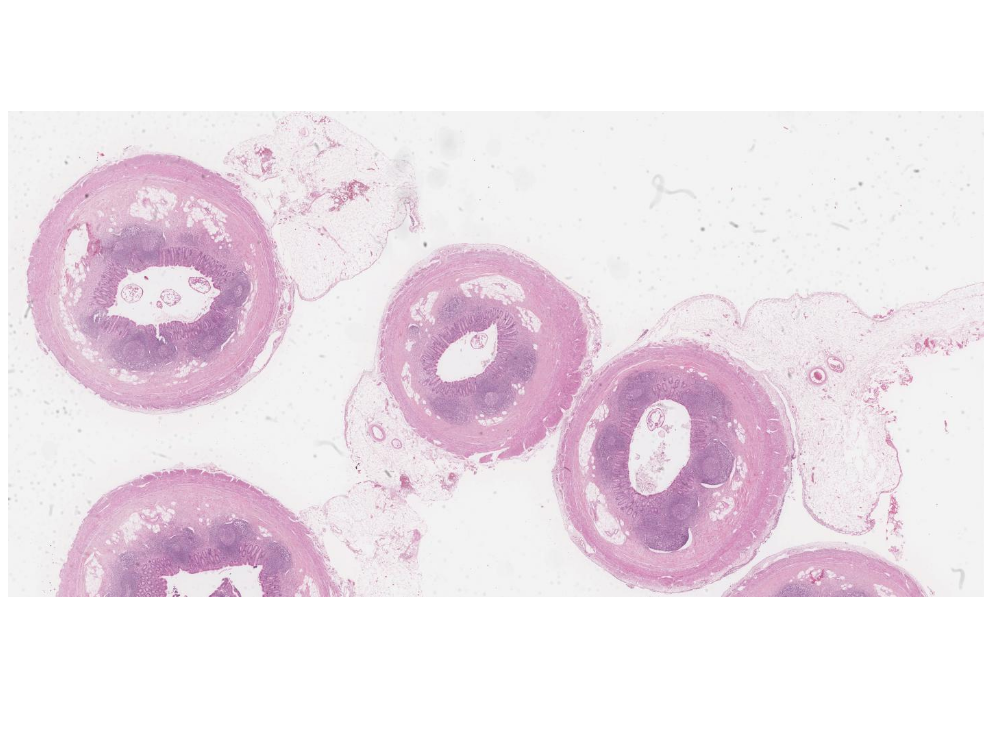
\includegraphics[width=0.25\textwidth,height=\textheight]{./screenshots/enterobius-vermicularis_screenshot.png}}
\href{https://images.patolojiatlasi.com/enterobius-vermicularis/HE.html}{Tam
Ekran Görmek İçin Resmi Tıklayın}

\part{Temel Tümör Patolojisi}

\hypertarget{sec-benign-tumorler}{%
\chapter{Benign Tümörler}\label{sec-benign-tumorler}}

\hypertarget{sec-adenomlar}{%
\section{Adenomlar}\label{sec-adenomlar}}

\hypertarget{sec-tubuler-adenom}{%
\subsection{Tübüler Adenom}\label{sec-tubuler-adenom}}

\hypertarget{sec-sesil-polip}{%
\subsubsection{Sesil Polip, Flat (Düz) Tübüler
Adenom}\label{sec-sesil-polip}}

\href{https://images.patolojiatlasi.com/tubularadenoma-flat/HE.html}{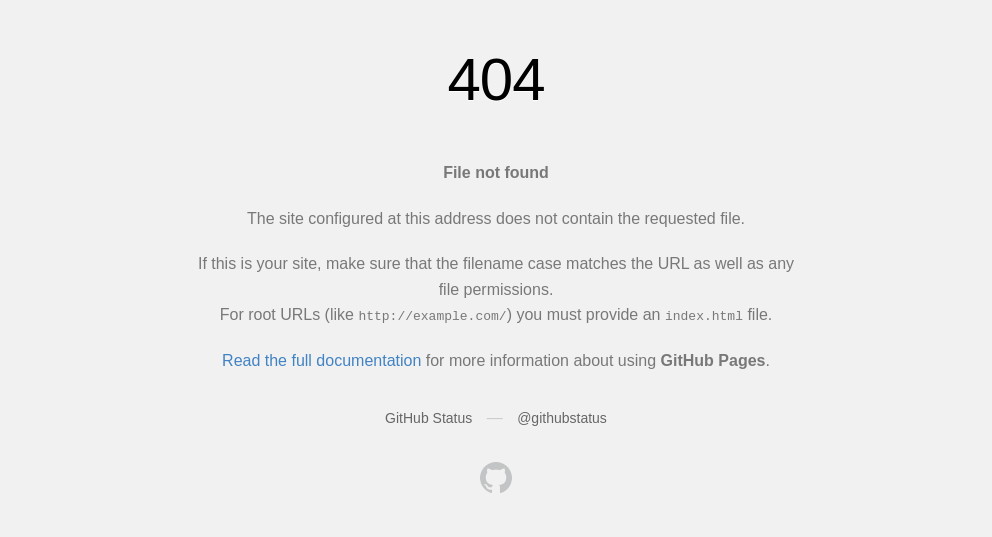
\includegraphics[width=0.25\textwidth,height=\textheight]{./screenshots/tubularadenoma-flat1_screenshot.png}}
\href{https://images.patolojiatlasi.com/tubularadenoma-flat/HE.html}{Tam
Ekran Görmek İçin Resmi Tıklayın}

\href{https://images.patolojiatlasi.com/tubularadenoma-flat/HE2.html}{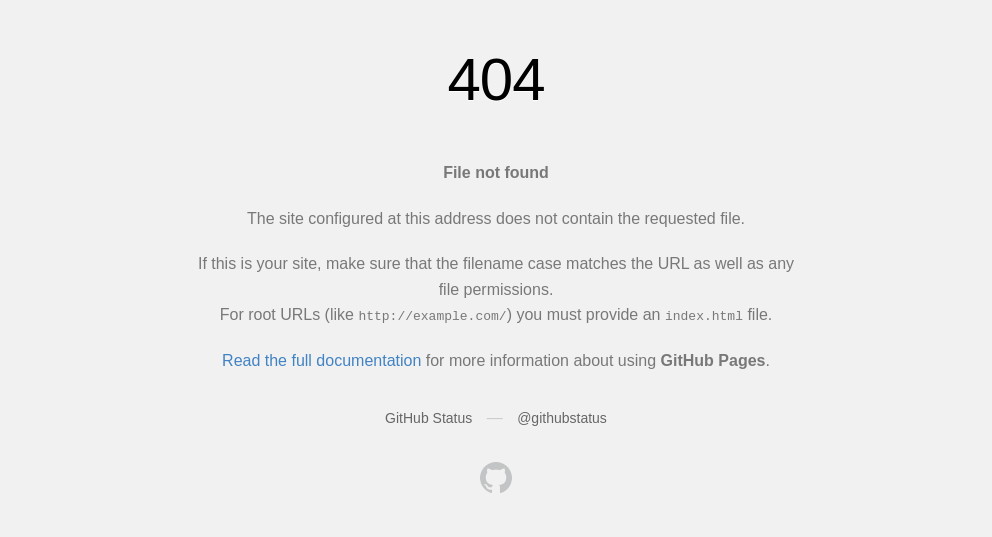
\includegraphics[width=0.25\textwidth,height=\textheight]{./screenshots/tubularadenoma-flat2_screenshot.png}}
\href{https://images.patolojiatlasi.com/tubularadenoma-flat/HE2.html}{Tam
Ekran Görmek İçin Resmi Tıklayın}

\hypertarget{sec-sapli-polip}{%
\subsubsection{Saplı Polip}\label{sec-sapli-polip}}

\hypertarget{sec-hamartom}{%
\chapter{Hamartom}\label{sec-hamartom}}

\hypertarget{sec-hamartomatoz-polip}{%
\section{Hamartomatöz Polip}\label{sec-hamartomatoz-polip}}

\href{https://images.patolojiatlasi.com/template/HE.html}{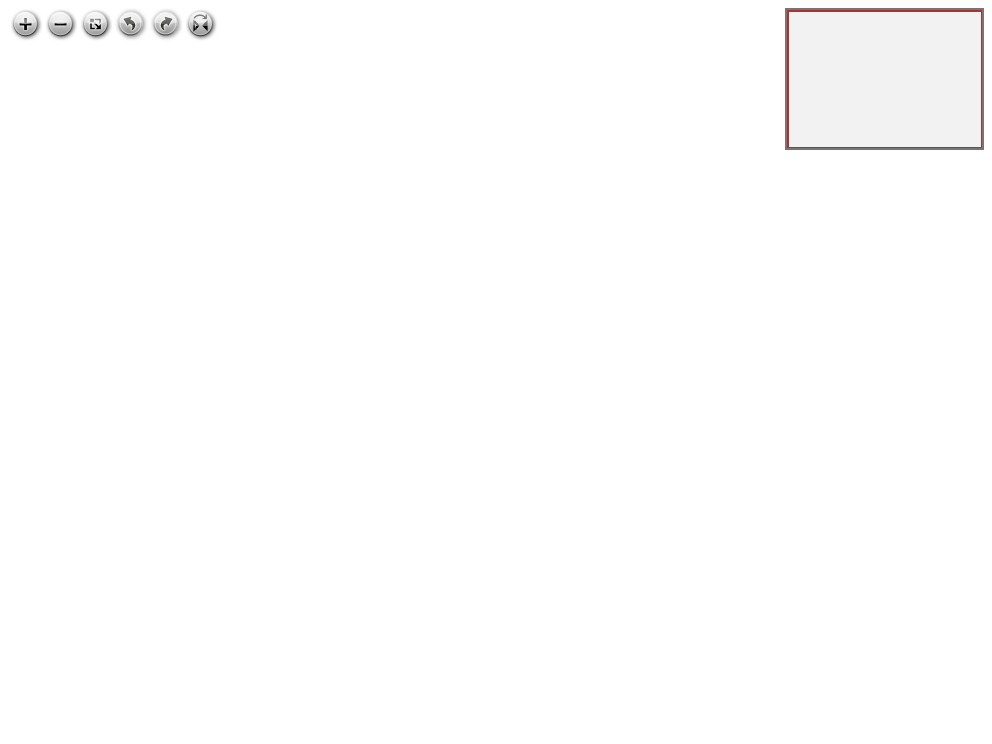
\includegraphics[width=0.25\textwidth,height=\textheight]{./screenshots/template_screenshot.png}}
\href{https://images.patolojiatlasi.com/hamartomatouspolyp/HE.html}{Tam
Ekran Görmek İçin Resmi Tıklayın}

\hypertarget{sec-schwann-cell-hamartoma-colon-polyp}{%
\section{Schwann Cell Hamartoma in a Colon
Polyp}\label{sec-schwann-cell-hamartoma-colon-polyp}}

\href{https://images.patolojiatlasi.com/template/HE.html}{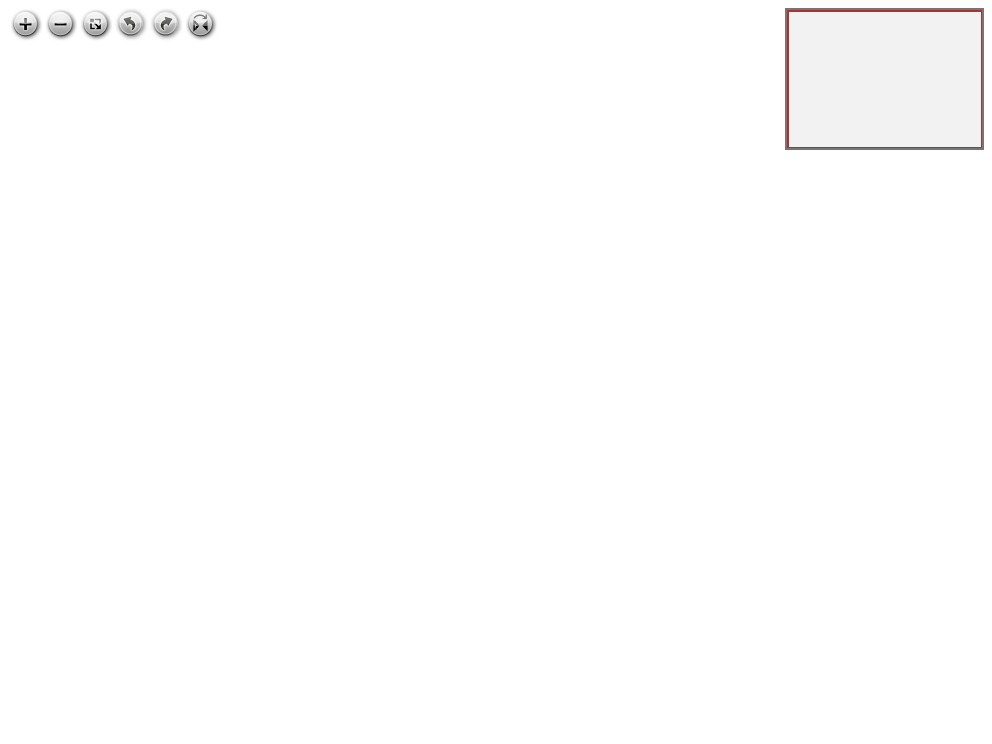
\includegraphics[width=0.25\textwidth,height=\textheight]{./screenshots/template_screenshot.png}}
\href{https://images.patolojiatlasi.com/schwanncellhamartoma/HE.html}{Tam
Ekran Görmek İçin Resmi Tıklayın}

\hypertarget{sec-heterotopi-ektopi}{%
\chapter{Heterotopi Ektopi}\label{sec-heterotopi-ektopi}}

\hypertarget{sec-intrapancreatic-spleen}{%
\section{Intrapancreatic Spleen,
Heterotopia}\label{sec-intrapancreatic-spleen}}

\href{https://images.patolojiatlasi.com/template/HE.html}{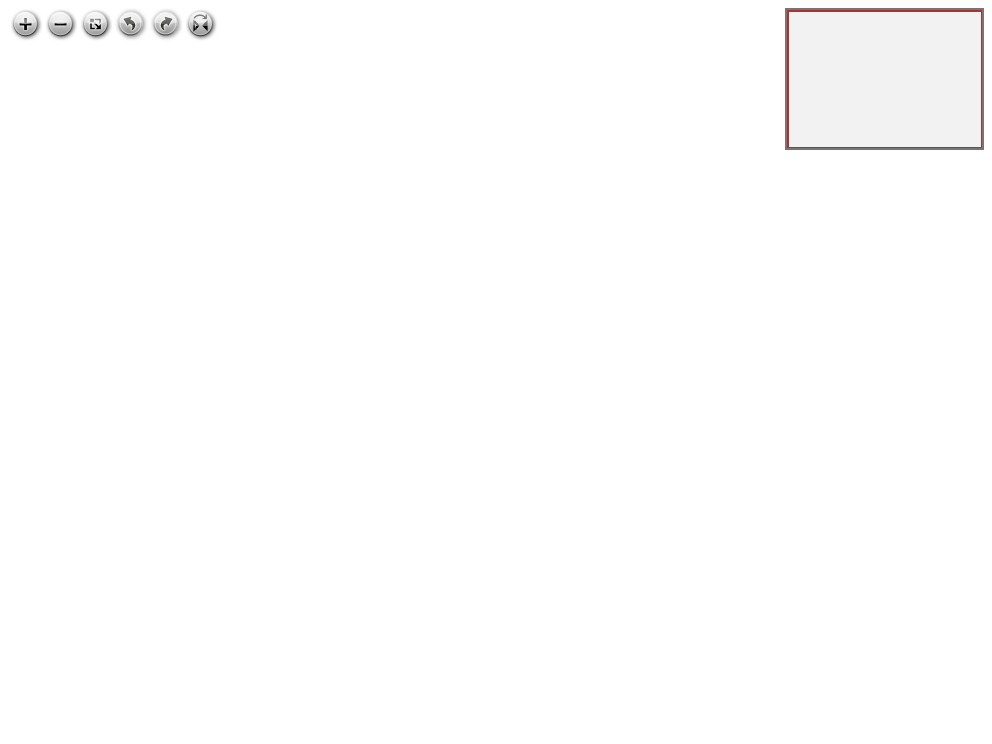
\includegraphics[width=0.25\textwidth,height=\textheight]{./screenshots/template_screenshot.png}}
\href{https://images.patolojiatlasi.com/intrapancreaticspleen/HE.html}{Tam
Ekran Görmek İçin Resmi Tıklayın}

\hypertarget{sec-paratubal-adneksiyal-bolgede-ektopik-adrenal}{%
\section{Paratubal adneksiyal bölgede ektopik adrenal
dokusu}\label{sec-paratubal-adneksiyal-bolgede-ektopik-adrenal}}

\textbf{Paratubal adneksiyal bölgede ektopik adrenal dokusu}

\href{https://images.patolojiatlasi.com/template/HE.html}{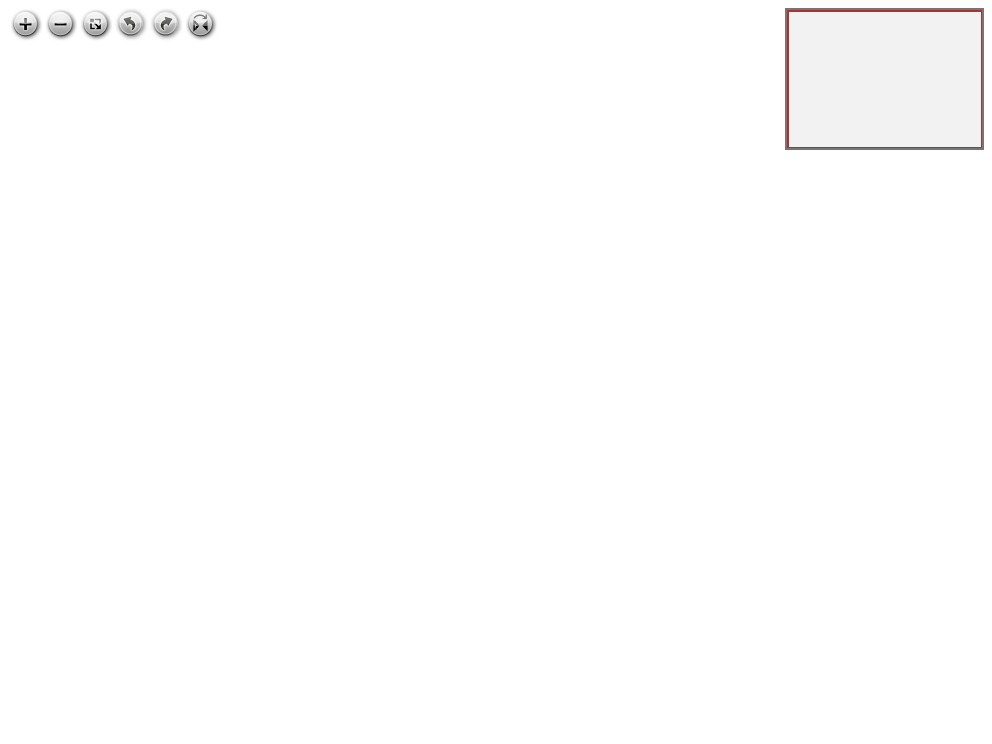
\includegraphics[width=0.25\textwidth,height=\textheight]{./screenshots/template_screenshot.png}}
\href{https://images.patolojiatlasi.com/ectopic-adrenal/HE.html}{Tam
Ekran Görmek İçin Resmi Tıklayın}

\hypertarget{sec-metaplazi}{%
\chapter{Metaplazi}\label{sec-metaplazi}}

\hypertarget{sec-pankreatik-asiner-metaplazi}{%
\section{Pankreatik Asiner Metaplazi,
Mide}\label{sec-pankreatik-asiner-metaplazi}}

\textbf{Pankreatik Asiner Metaplazi, Mide}

\href{https://images.patolojiatlasi.com/template/HE.html}{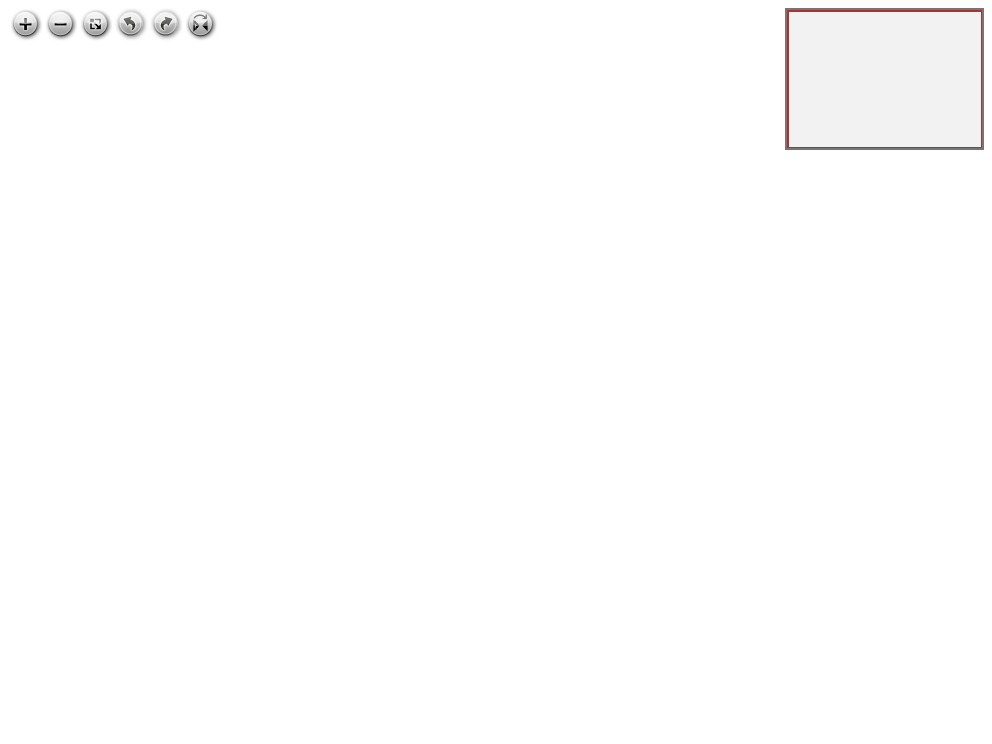
\includegraphics[width=0.25\textwidth,height=\textheight]{./screenshots/template_screenshot.png}}
\href{https://images.patolojiatlasi.com/metaplasia/HE.html}{Tam Ekran
Görmek İçin Resmi Tıklayın}

\hypertarget{sec-karsinogenez}{%
\chapter{Karsinogenez}\label{sec-karsinogenez}}

\hypertarget{sec-mepaplazi-displazi-karsinom}{%
\section{metaplazi, displazi,
karsinom}\label{sec-mepaplazi-displazi-karsinom}}

\textbf{metaplazi, displazi, karsinom}

\href{https://images.patolojiatlasi.com/template/HE.html}{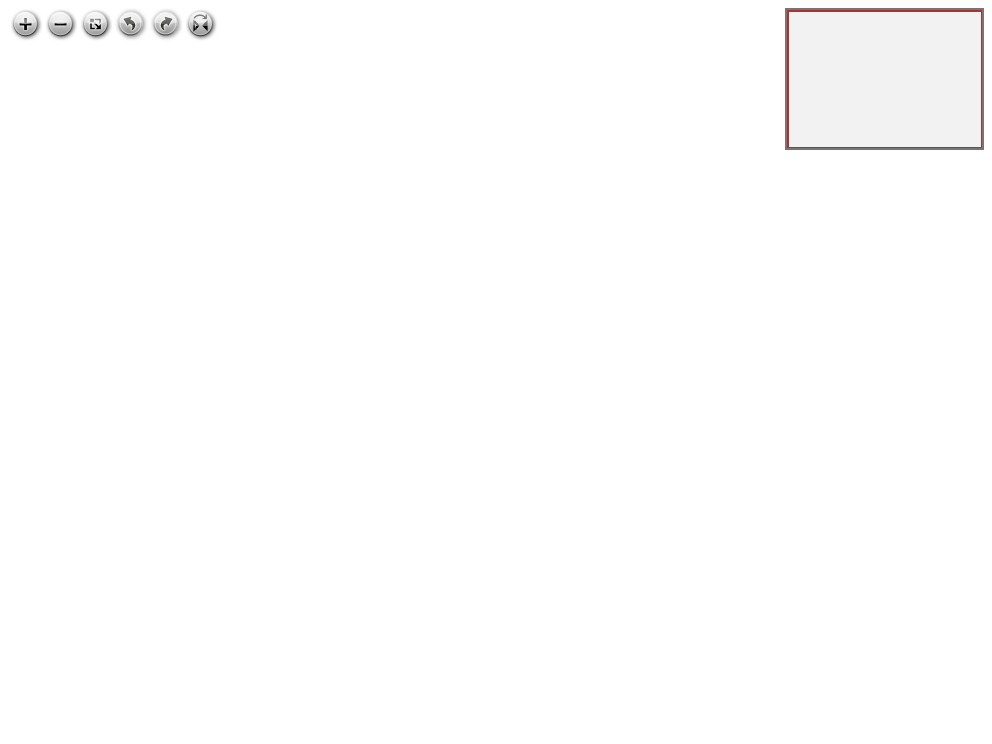
\includegraphics[width=0.25\textwidth,height=\textheight]{./screenshots/template_screenshot.png}}
\href{https://images.patolojiatlasi.com/carcinogenesis/HE.html}{Tam
Ekran Görmek İçin Resmi Tıklayın}

\hypertarget{sec-malign-tumor-ozellikleri}{%
\chapter{Malign Tümör Özellikleri}\label{sec-malign-tumor-ozellikleri}}

\hypertarget{sec-pleomorfizm}{%
\section{Pleomorfizm}\label{sec-pleomorfizm}}

\textbf{Pleomorfizm}

\href{https://images.patolojiatlasi.com/template/HE.html}{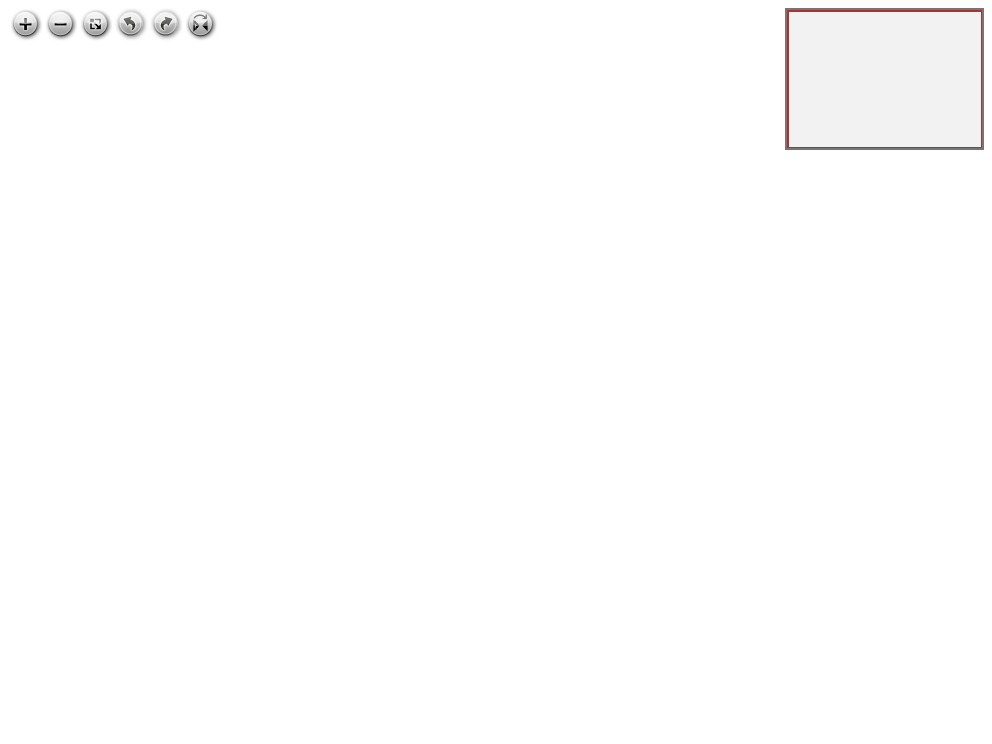
\includegraphics[width=0.25\textwidth,height=\textheight]{./screenshots/template_screenshot.png}}
\href{https://images.patolojiatlasi.com/pleomorphism/HE.html}{Tam Ekran
Görmek İçin Resmi Tıklayın}

\hypertarget{sec-metastaz}{%
\chapter{Metastaz}\label{sec-metastaz}}

\hypertarget{sec-karaciger-sarkom-metastaz}{%
\section{Karaciğerde Sarkom
Metastazı}\label{sec-karaciger-sarkom-metastaz}}

\href{https://images.patolojiatlasi.com/template/HE.html}{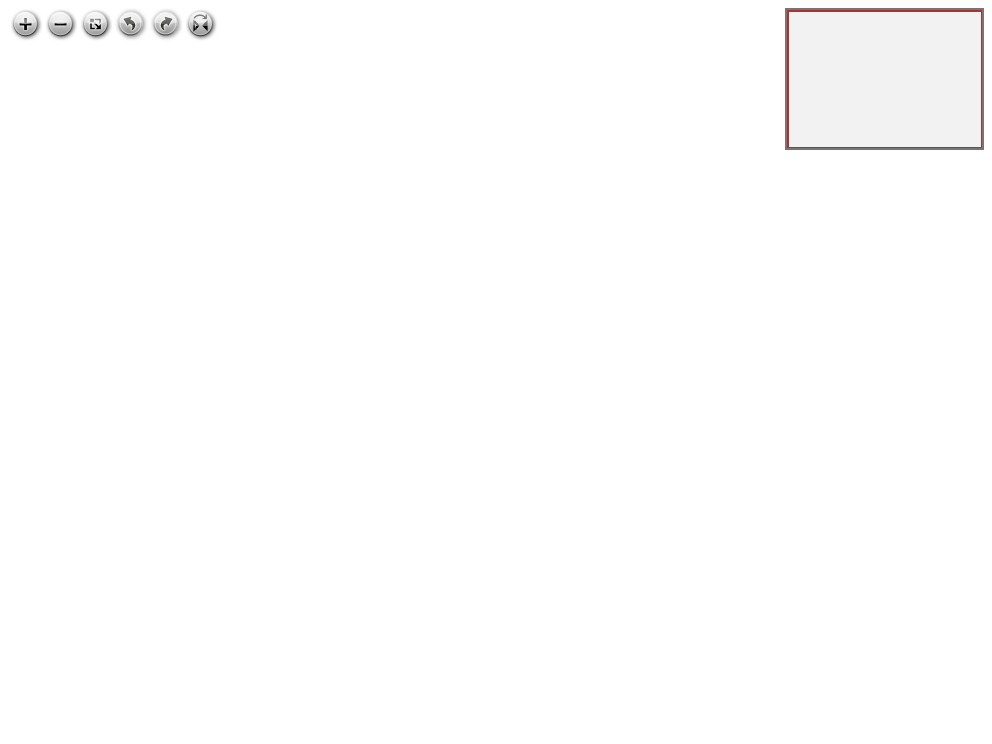
\includegraphics[width=0.25\textwidth,height=\textheight]{./screenshots/template_screenshot.png}}
\href{https://images.patolojiatlasi.com/metastaticsarcoma/HE.html}{Tam
Ekran Görmek İçin Resmi Tıklayın}

\hypertarget{sec-sinsi-lenf-nodu-metastazi}{%
\section{Sinsi bir lenf nodu
metastazı}\label{sec-sinsi-lenf-nodu-metastazi}}

\textbf{Sinsi bir lenf nodu metastazı HE}

\href{https://images.patolojiatlasi.com/template/HE.html}{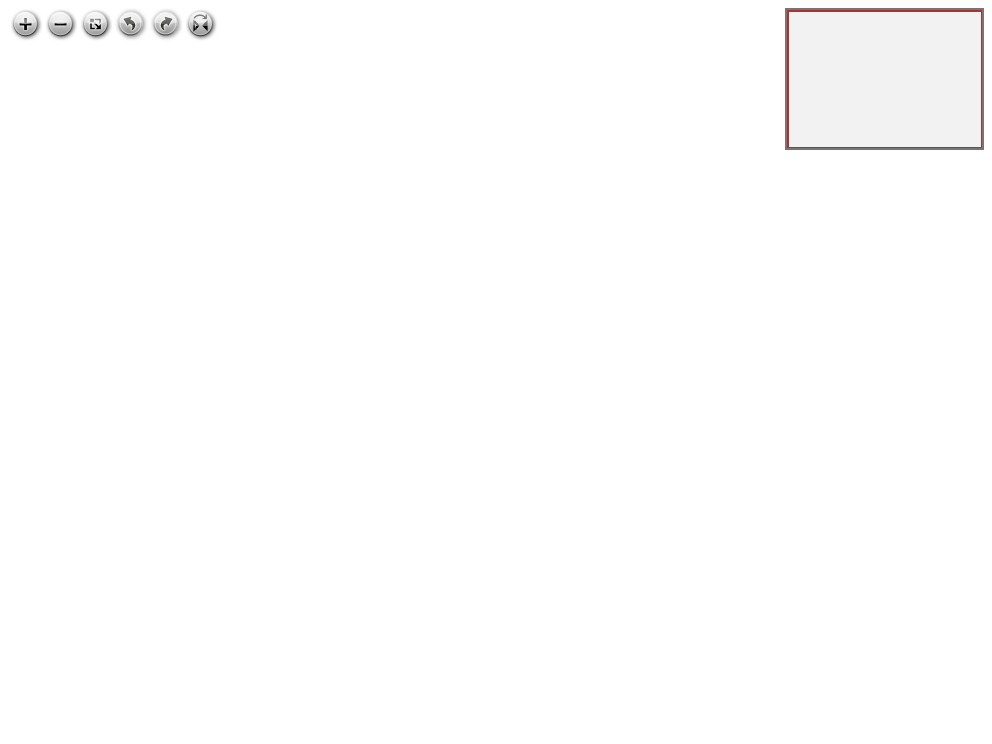
\includegraphics[width=0.25\textwidth,height=\textheight]{./screenshots/template_screenshot.png}}
\href{https://images.patolojiatlasi.com/insidious-lymph-node-metastasis/HE.html}{Tam
Ekran Görmek İçin Resmi Tıklayın}

\textbf{Sinsi bir lenf nodu metastazı OSKAR panCK}

\href{https://images.patolojiatlasi.com/template/HE.html}{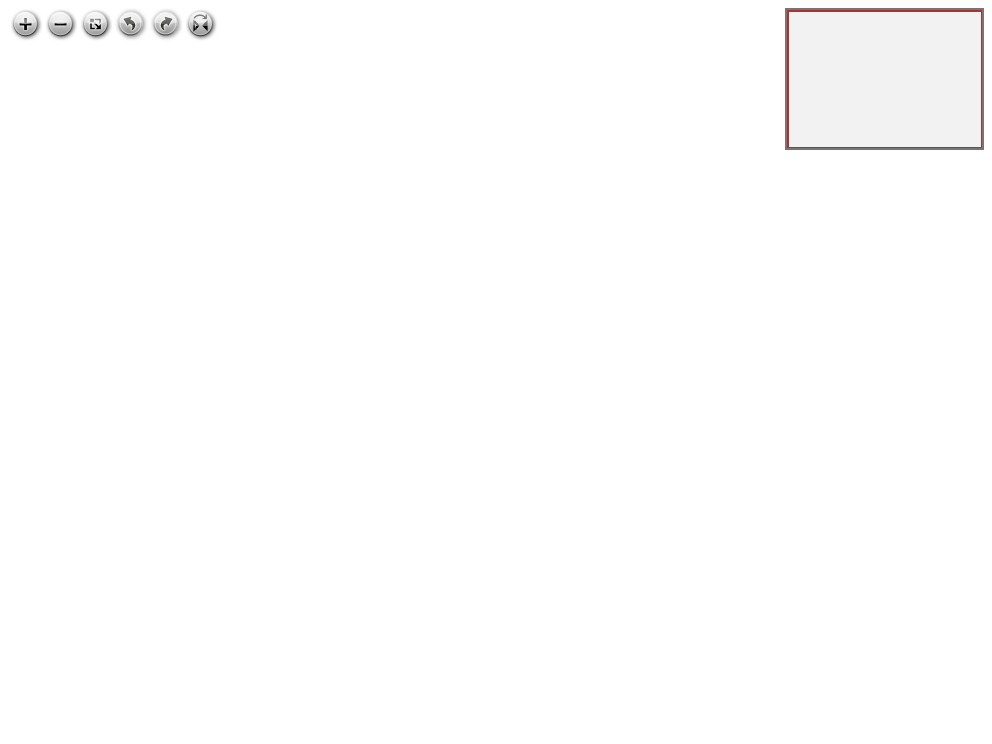
\includegraphics[width=0.25\textwidth,height=\textheight]{./screenshots/template_screenshot.png}}
\href{https://images.patolojiatlasi.com/insidious-lymph-node-metastasis/OSKARCK.html}{Tam
Ekran Görmek İçin Resmi Tıklayın}

\hypertarget{sec-baska-organlara-tumor-yayilimi}{%
\chapter{Başka Organlara Tümör
Yayılımı}\label{sec-baska-organlara-tumor-yayilimi}}

\hypertarget{sec-servikse-kolon-tumor-yayilimi}{%
\section{Servikse kolon tümörü
yayılımı}\label{sec-servikse-kolon-tumor-yayilimi}}

\textbf{Servikse kolon tümörü yayılımı}

\href{https://images.patolojiatlasi.com/tumor-spread/HE-cervix.html}{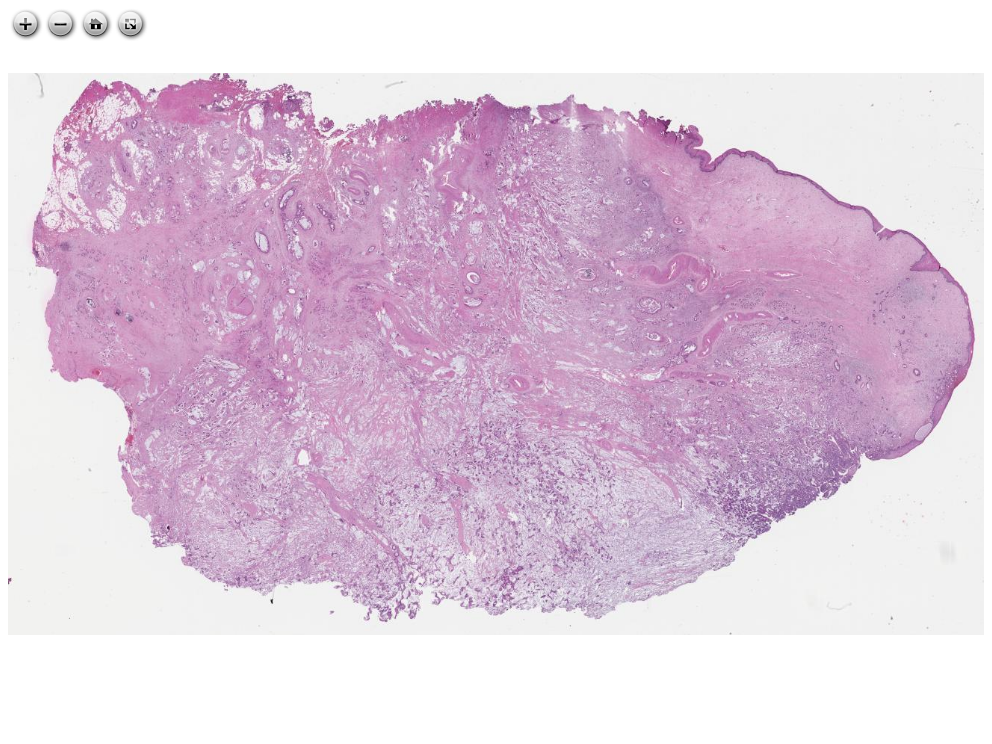
\includegraphics[width=0.25\textwidth,height=\textheight]{./screenshots/tumor-spread-cervix_screenshot.png}}
\href{https://images.patolojiatlasi.com/tumor-spread/HE-cervix.html}{Tam
Ekran Görmek İçin Resmi Tıklayın}

\hypertarget{sec-endometriuma-kolon-tumor-yayilimi}{%
\section{Endometriuma kolon tümörü
yayılımı}\label{sec-endometriuma-kolon-tumor-yayilimi}}

\textbf{Endometriuma kolon tümörü yayılımı}

\href{https://images.patolojiatlasi.com/tumor-spread/HE-endometrium.html}{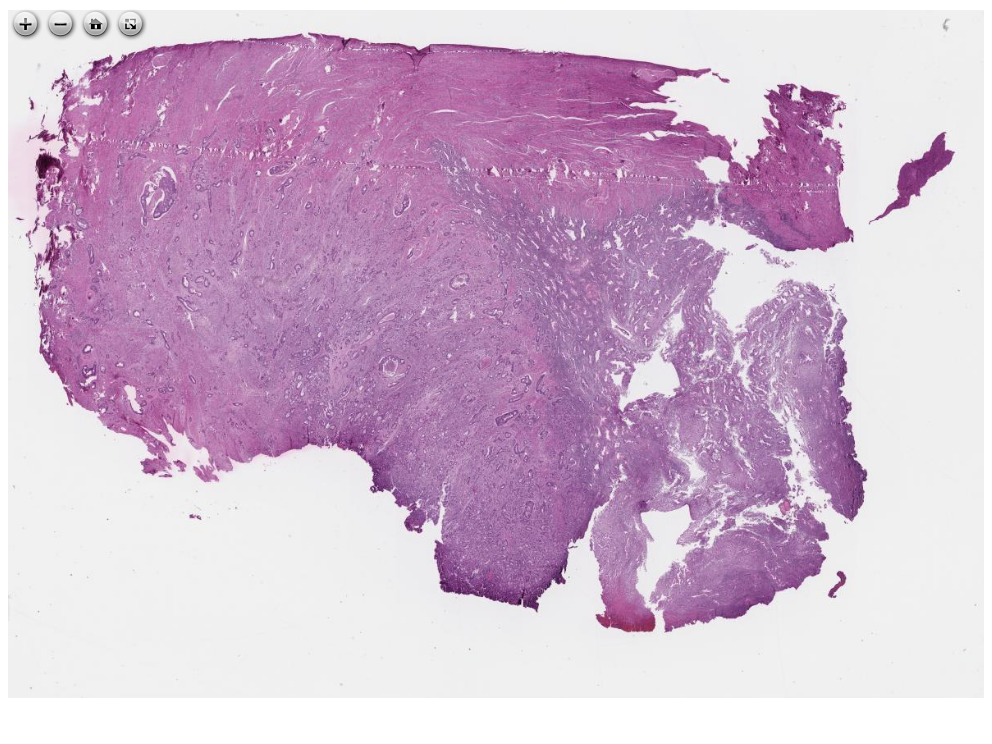
\includegraphics[width=0.25\textwidth,height=\textheight]{./screenshots/tumor-spread-endometrium_screenshot.png}}
\href{https://images.patolojiatlasi.com/tumor-spread/HE-endometrium.html}{Tam
Ekran Görmek İçin Resmi Tıklayın}

\hypertarget{sec-overe-kolon-tumor-yayilimi}{%
\section{Overe kolon tümörü
yayılımı}\label{sec-overe-kolon-tumor-yayilimi}}

\textbf{Overe kolon tümörü yayılımı}

\href{https://images.patolojiatlasi.com/tumor-spread/HE-over.html}{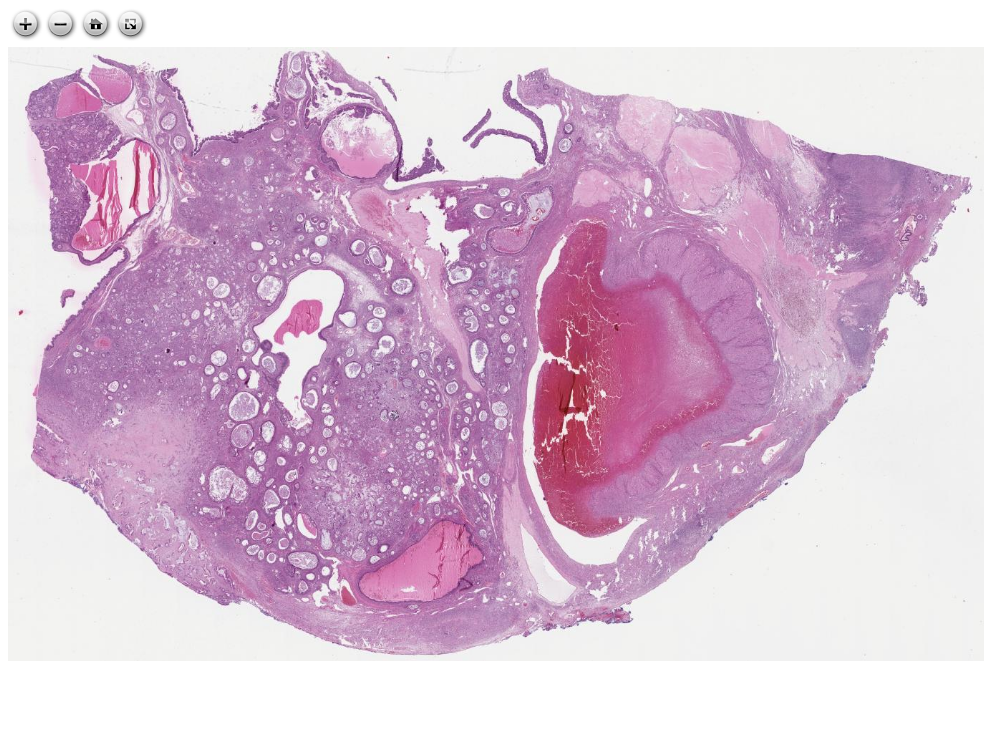
\includegraphics[width=0.25\textwidth,height=\textheight]{./screenshots/tumor-spread-over_screenshot.png}}
\href{https://images.patolojiatlasi.com/tumor-spread/HE-over.html}{Tam
Ekran Görmek İçin Resmi Tıklayın}

\hypertarget{sec-ince-barsak-kolon-tumor-yayilimi}{%
\section{İnce barsağa kolon tümörü
yayılımı}\label{sec-ince-barsak-kolon-tumor-yayilimi}}

\textbf{İnce barsağa kolon tümörü yayılımı}

\href{https://images.patolojiatlasi.com/tumor-spread/HE-small-intestine.html}{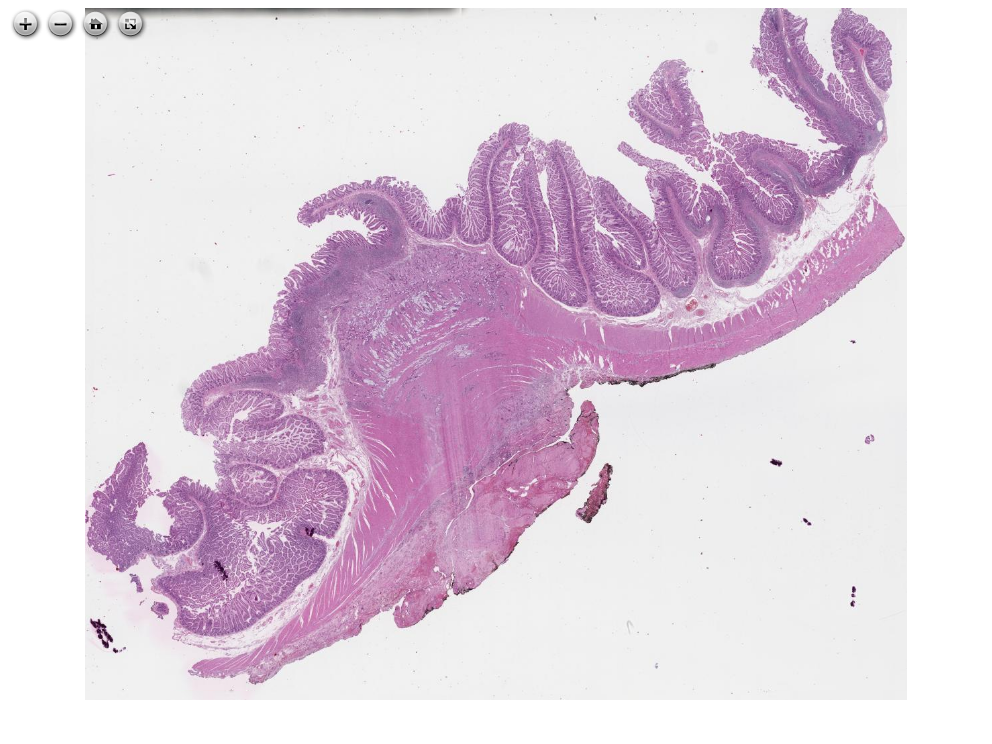
\includegraphics[width=0.25\textwidth,height=\textheight]{./screenshots/tumor-spread-small-intestine_screenshot.png}}
\href{https://images.patolojiatlasi.com/tumor-spread/HE-small-intestine.html}{Tam
Ekran Görmek İçin Resmi Tıklayın}

\part{Tümörlerdeki Prognostik Morfolojik Özellikler}

\hypertarget{sec-venoz-invazyon}{%
\chapter{Venöz invazyon}\label{sec-venoz-invazyon}}

\textbf{Venöz invazyon}

\href{https://images.patolojiatlasi.com/venous-invasion/HE.html}{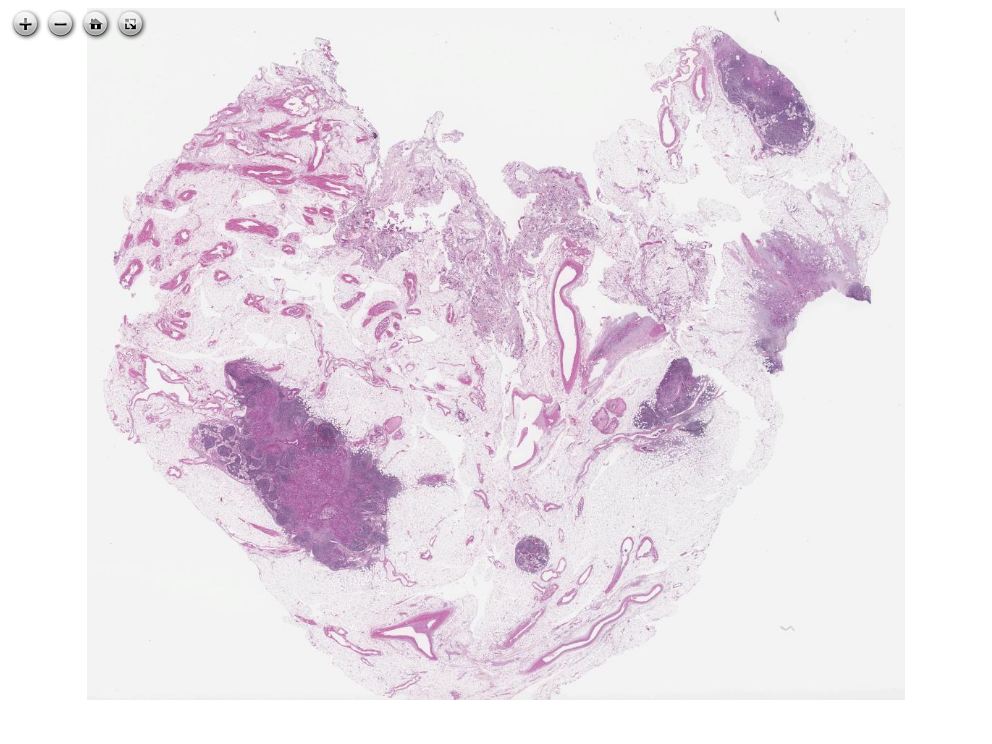
\includegraphics[width=0.25\textwidth,height=\textheight]{./screenshots/venous-invasion_screenshot.png}}
\href{https://images.patolojiatlasi.com/venous-invasion/HE.html}{Tam
Ekran Görmek İçin Resmi Tıklayın}

\hypertarget{sec-adenokarsinomda-ekstramural-venoz-invazyon}{%
\chapter{Adenokarsinomda Ekstramural Venöz
İnvazyon}\label{sec-adenokarsinomda-ekstramural-venoz-invazyon}}

\textbf{Adenokarsinomda Ekstramural Venöz İnvazyon}

\href{https://images.patolojiatlasi.com/extramuralvenousinvasion/HE.html}{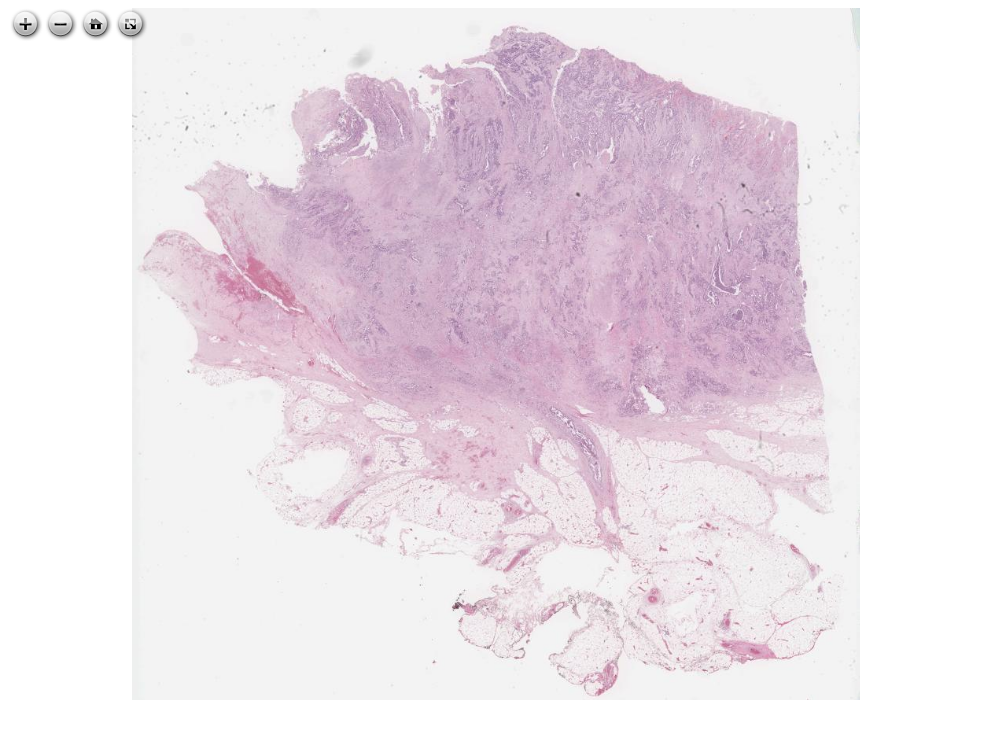
\includegraphics[width=0.25\textwidth,height=\textheight]{./screenshots/extramuralvenousinvasion_screenshot.png}}
\href{https://images.patolojiatlasi.com/extramuralvenousinvasion/HE.html}{Tam
Ekran Görmek İçin Resmi Tıklayın}

\textbf{ekstramural venöz invazyon}

\href{https://images.patolojiatlasi.com/extramural-venous-invasion/HE.html}{\includegraphics[width=0.25\textwidth,height=\textheight]{./screenshots/extramural-venous-invasion_screenshot.png}}
\href{https://images.patolojiatlasi.com/extramural-venous-invasion/HE.html}{Tam
Ekran Görmek İçin Resmi Tıklayın}

\part{Hematopatoloji}

\hypertarget{sec-hodgkin-lenfoma}{%
\chapter{Hodgkin Lenfoma}\label{sec-hodgkin-lenfoma}}

\textbf{Hodgkin Lenfoma}

\href{https://images.patolojiatlasi.com/template/HE.html}{\includegraphics[width=0.25\textwidth,height=\textheight]{./screenshots/template_screenshot.png}}
\href{https://images.patolojiatlasi.com/hodgkin/HE.html}{Tam Ekran
Görmek İçin Resmi Tıklayın}

\part{Gastrointestinal Sistem Patolojisi}

\hypertarget{sec-gastrointestinal-sistem}{%
\chapter{Gastrointestinal Sistem}\label{sec-gastrointestinal-sistem}}

\hypertarget{sec-ozofagus}{%
\chapter{Özofagus}\label{sec-ozofagus}}

\hypertarget{sec-ozofagus-granuler-hucreli-tumor}{%
\section{Özofagusta Granüler Hücreli
Tümör}\label{sec-ozofagus-granuler-hucreli-tumor}}

\textbf{Özofagusta Granüler Hücreli Tümör}

\href{https://images.patolojiatlasi.com/granular-cell-tumor/HE.html}{\includegraphics[width=0.25\textwidth,height=\textheight]{./screenshots/granular-cell-tumor_screenshot.png}}
\href{https://images.patolojiatlasi.com/granular-cell-tumor/HE.html}{Tam
Ekran Görmek İçin Resmi Tıklayın}

\hypertarget{sec-mide-patolojisi}{%
\chapter{Mide Patolojisi}\label{sec-mide-patolojisi}}

\hypertarget{sec-gastritis-cystica-profunda}{%
\section{Gastritis Cystica
Profunda}\label{sec-gastritis-cystica-profunda}}

\textbf{Gastritis Cystica Profunda}

\href{https://images.patolojiatlasi.com/gastritis-cystica-profunda/HE.html}{\includegraphics[width=0.25\textwidth,height=\textheight]{./screenshots/gastritis-cystica-profunda_screenshot.png}}
\href{https://images.patolojiatlasi.com/gastritis-cystica-profunda/HE.html}{Tam
Ekran Görmek İçin Resmi Tıklayın}

\hypertarget{lymphocytic-gastritis}{%
\chapter{lymphocytic-gastritis}\label{lymphocytic-gastritis}}

\textbf{lymphocytic-gastritis for pathology atlas repositories}

\hypertarget{sec-lymphocytic-gastritis}{%
\section{lenfositik gastrit}\label{sec-lymphocytic-gastritis}}

\textbf{lenfositik gastrit HE}

\href{https://images.patolojiatlasi.com/lymphocytic-gastritis/HE.html}{\includegraphics[width=0.25\textwidth,height=\textheight]{./screenshots/lymphocytic-gastritisHE_screenshot.png}}
\href{https://images.patolojiatlasi.com/lymphocytic-gastritis/HE.html}{Tam
Ekran Görmek İçin Resmi Tıklayın}

\textbf{lenfositik gastrit CD3}

\href{https://images.patolojiatlasi.com/lymphocytic-gastritis/CD3.html}{\includegraphics[width=0.25\textwidth,height=\textheight]{./screenshots/lymphocytic-gastritisCD3_screenshot.png}}
\href{https://images.patolojiatlasi.com/lymphocytic-gastritis/CD3.html}{Tam
Ekran Görmek İçin Resmi Tıklayın}

\textbf{lenfositik gastrit CD8}

\href{https://images.patolojiatlasi.com/lymphocytic-gastritis/CD8.html}{\includegraphics[width=0.25\textwidth,height=\textheight]{./screenshots/lymphocytic-gastritisCD8_screenshot.png}}
\href{https://images.patolojiatlasi.com/lymphocytic-gastritis/CD8.html}{Tam
Ekran Görmek İçin Resmi Tıklayın}

\textbf{lenfositik gastrit CD20}

\href{https://images.patolojiatlasi.com/lymphocytic-gastritis/CD20.html}{\includegraphics[width=0.25\textwidth,height=\textheight]{./screenshots/lymphocytic-gastritisCD20_screenshot.png}}
\href{https://images.patolojiatlasi.com/lymphocytic-gastritis/CD20.html}{Tam
Ekran Görmek İçin Resmi Tıklayın}

\hypertarget{sec-duodenum}{%
\chapter{Duodenum}\label{sec-duodenum}}

\hypertarget{sec-colyak-hastaligi}{%
\section{Çölyak Hastalığı}\label{sec-colyak-hastaligi}}

\textbf{Çölyak Hastalığı}

\href{https://images.patolojiatlasi.com/celiac-disease/HE.html}{\includegraphics[width=0.25\textwidth,height=\textheight]{./screenshots/celiac-disease_screenshot.png}}
\href{https://images.patolojiatlasi.com/celiac-disease/HE.html}{Tam
Ekran Görmek İçin Resmi Tıklayın}

\hypertarget{kolon-patolojisi}{%
\chapter{Kolon Patolojisi}\label{kolon-patolojisi}}

\hypertarget{sec-iskemik-kolit}{%
\section{İskemik Kolit}\label{sec-iskemik-kolit}}

\textbf{İskemik Kolit}

\href{https://images.patolojiatlasi.com/template/HE.html}{\includegraphics[width=0.25\textwidth,height=\textheight]{./screenshots/template_screenshot.png}}
\href{https://images.patolojiatlasi.com/ischemic-colitis/HE.html}{Tam
Ekran Görmek İçin Resmi Tıklayın}

\hypertarget{sec-kolon-benign-tumorler}{%
\section{Benign Tümörler}\label{sec-kolon-benign-tumorler}}

\hypertarget{sec-kolon-tubuler-adenom}{%
\subsection{Tübüler Adenom}\label{sec-kolon-tubuler-adenom}}

\hypertarget{sec-kolon-sesil-polip}{%
\subsubsection{Sesil Polip, Flat (Düz) Tübüler
Adenom}\label{sec-kolon-sesil-polip}}

\href{https://images.patolojiatlasi.com/tubularadenoma-flat/HE.html}{\includegraphics[width=0.25\textwidth,height=\textheight]{./screenshots/tubularadenoma-flat1_screenshot.png}}
\href{https://images.patolojiatlasi.com/tubularadenoma-flat/HE.html}{Tam
Ekran Görmek İçin Resmi Tıklayın}

\href{https://images.patolojiatlasi.com/tubularadenoma-flat/HE2.html}{\includegraphics[width=0.25\textwidth,height=\textheight]{./screenshots/tubularadenoma-flat2_screenshot.png}}
\href{https://images.patolojiatlasi.com/tubularadenoma-flat/HE2.html}{Tam
Ekran Görmek İçin Resmi Tıklayın}

\hypertarget{sec-kolon-sapli-polip}{%
\subsubsection{Saplı Polip}\label{sec-kolon-sapli-polip}}

Macroscopy

\href{https://images.patolojiatlasi.com/tubularadenoma/tubular-adenoma-with-stalk-macroscopy.jpg}{tubular
adenoma with a stalk macroscopy}

\begin{figure}

{\centering \includegraphics{index_files/mediabag/tubular-adenoma-with.jpg}

}

\caption{saplı polip}

\end{figure}

Microscopy

\href{https://images.patolojiatlasi.com/tubularadenoma/tubular-adenoma-with-stalk.jpeg}{tubular
adenoma with a stalk}

\hypertarget{sec-kolon-hiperplastik-polip}{%
\subsection{Hiperplastik Polip}\label{sec-kolon-hiperplastik-polip}}

Mikroskopi

\href{https://images.patolojiatlasi.com/template/HE.html}{\includegraphics[width=0.25\textwidth,height=\textheight]{./screenshots/template_screenshot.png}}
\href{https://images.patolojiatlasi.com/hyperplasticpolyp/case1.html}{Tam
Ekran Görmek İçin Resmi Tıklayın}

\hypertarget{sec-kolon-hamartomatoz-polip}{%
\subsection{Hamartomatöz Polip}\label{sec-kolon-hamartomatoz-polip}}

\href{https://images.patolojiatlasi.com/template/HE.html}{\includegraphics[width=0.25\textwidth,height=\textheight]{./screenshots/template_screenshot.png}}
\href{https://images.patolojiatlasi.com/hamartomatouspolyp/HE.html}{Tam
Ekran Görmek İçin Resmi Tıklayın}

\hypertarget{sec-colon-schwann-cell-hamartoma}{%
\subsubsection{Schwann Cell Hamartoma in a Colon
Polyp}\label{sec-colon-schwann-cell-hamartoma}}

\href{https://images.patolojiatlasi.com/template/HE.html}{\includegraphics[width=0.25\textwidth,height=\textheight]{./screenshots/template_screenshot.png}}
\href{https://images.patolojiatlasi.com/schwanncellhamartoma/HE.html}{Tam
Ekran Görmek İçin Resmi Tıklayın}

\hypertarget{sec-kolon-intramukozal-lipom}{%
\chapter{Kolon submukozal lipom}\label{sec-kolon-intramukozal-lipom}}

\textbf{Kolon submukozal lipom}

\href{https://images.patolojiatlasi.com/template/HE.html}{\includegraphics[width=0.25\textwidth,height=\textheight]{./screenshots/template_screenshot.png}}
\href{https://images.patolojiatlasi.com/colon-submucosal-lipoma/HE.html}{Tam
Ekran Görmek İçin Resmi Tıklayın}

\hypertarget{sec-tubulovilloz-adenom-zemininde-adenokarsinom}{%
\chapter{Tübülövillöz adenom zemininde gelişmiş Müsinöz adenokarsinom,
kolon}\label{sec-tubulovilloz-adenom-zemininde-adenokarsinom}}

\textbf{Tübülövillöz adenom zemininde gelişmiş Müsinöz adenokarsinom,
kolon}

\href{https://images.patolojiatlasi.com/template/HE.html}{\includegraphics[width=0.25\textwidth,height=\textheight]{./screenshots/template_screenshot.png}}
\href{https://images.patolojiatlasi.com/mucinous-adenocarcinoma-colon/HE.html}{Tam
Ekran Görmek İçin Resmi Tıklayın}

\begin{center}\rule{0.5\linewidth}{0.5pt}\end{center}

\hypertarget{sec-kolon-adenokarsinomu}{%
\chapter{Kolon Adenokarsinomu}\label{sec-kolon-adenokarsinomu}}

\textbf{Kolon Adenokarsinomu}

\href{https://images.patolojiatlasi.com/template/HE.html}{\includegraphics[width=0.25\textwidth,height=\textheight]{./screenshots/template_screenshot.png}}
\href{https://images.patolojiatlasi.com/colon-adenocarcinoma/HE.html}{Tam
Ekran Görmek İçin Resmi Tıklayın}

\textbf{Kolon Adenokarsinomu}

\href{https://images.patolojiatlasi.com/template/HE.html}{\includegraphics[width=0.25\textwidth,height=\textheight]{./screenshots/template_screenshot.png}}
\href{https://images.patolojiatlasi.com/colon-adenocarcinoma/HE2.html}{Tam
Ekran Görmek İçin Resmi Tıklayın}

\textbf{Kolon Adenokarsinomu pT4a}

\href{https://images.patolojiatlasi.com/template/HE.html}{\includegraphics[width=0.25\textwidth,height=\textheight]{./screenshots/template_screenshot.png}}
\href{https://images.patolojiatlasi.com/colon-adenocarcinoma/HE3.html}{Tam
Ekran Görmek İçin Resmi Tıklayın}

\part{Karaciğer Patolojisi}

\hypertarget{sec-karaciger-tumorleri}{%
\chapter{Karaciğer Tümörleri}\label{sec-karaciger-tumorleri}}

\hypertarget{sec-hepatoseluler-karsinom}{%
\section{Hepatoselüler Karsinom}\label{sec-hepatoseluler-karsinom}}

\href{https://images.patolojiatlasi.com/template/HE.html}{\includegraphics[width=0.25\textwidth,height=\textheight]{./screenshots/template_screenshot.png}}
\href{https://images.patolojiatlasi.com/hepatocellularcarcinoma/HCC/viewer_z0.html}{Tam
Ekran Görmek İçin Resmi Tıklayın}

\hypertarget{sec-hepatoseluler-karsinom-fibrolamellar}{%
\section{Hepatoselüler karsinom,
fibrolamellar}\label{sec-hepatoseluler-karsinom-fibrolamellar}}

\textbf{Hepatoselüler karsinom, fibrolamellar}

\href{https://images.patolojiatlasi.com/template/HE.html}{\includegraphics[width=0.25\textwidth,height=\textheight]{./screenshots/template_screenshot.png}}
\href{https://images.patolojiatlasi.com/fibrolamellar-hepatocellular-carcinoma/HE1.html}{Tam
Ekran Görmek İçin Resmi Tıklayın}

\href{https://images.patolojiatlasi.com/template/HE.html}{\includegraphics[width=0.25\textwidth,height=\textheight]{./screenshots/template_screenshot.png}}
\href{https://images.patolojiatlasi.com/fibrolamellar-hepatocellular-carcinoma/HE4.html}{Click
for Full Screen WSI}

\hypertarget{sec-benign-karaciger-tumorleri}{%
\chapter{Benign Karaciğer
Tümörleri}\label{sec-benign-karaciger-tumorleri}}

\hypertarget{sec-karaciger-hemanjiom}{%
\section{Karaciğer Hemanjiom}\label{sec-karaciger-hemanjiom}}

\textbf{Karaciğer Hemanjiom}

\href{https://images.patolojiatlasi.com/liver-hemangioma/HE.html}{\includegraphics[width=0.25\textwidth,height=\textheight]{./screenshots/liver-hemangioma_screenshot.png}}
\href{https://images.patolojiatlasi.com/liver-hemangioma/HE.html}{Tam
Ekran Görmek İçin Resmi Tıklayın}

\part{Pankreatobilier Sistem Patolojisi}

\hypertarget{sec-pankreas-tumorleri}{%
\chapter{Pankreas Tümörleri}\label{sec-pankreas-tumorleri}}

\hypertarget{sec-pankreas-musinous-adenokarsinom-osteoklast}{%
\section{pankreas, müsinöz adenokarsinom zemininde gelişmiş, osteoklast
benzeri dev hücreler içeren indiferansiye
karsinom}\label{sec-pankreas-musinous-adenokarsinom-osteoklast}}

\textbf{pankreas, müsinöz adenokarsinom zemininde gelişmiş, osteoklast
benzeri dev hücreler içeren indiferansiye karsinom}

\href{https://images.patolojiatlasi.com/pancreas-undifferentiated-osteoclast/HE.html}{\includegraphics[width=0.25\textwidth,height=\textheight]{./screenshots/pancreas-undifferentiated-osteoclast_screenshot.png}}
\href{https://images.patolojiatlasi.com/pancreas-undifferentiated-osteoclast/HE.html}{Tam
Ekran Görmek İçin Resmi Tıklayın}

\hypertarget{sec-safra-kesesi}{%
\chapter{Safra Kesesi}\label{sec-safra-kesesi}}

\hypertarget{sec-safra-kesesi-adenomyom}{%
\section{Safra Kesesi Adenomyom}\label{sec-safra-kesesi-adenomyom}}

\textbf{Safra Kesesi Adenomyom}

\href{https://images.patolojiatlasi.com/gallbladder-adenomyoma/HE.html}{\includegraphics[width=0.25\textwidth,height=\textheight]{./screenshots/gallbladder-adenomyoma_screenshot.png}}
\href{https://images.patolojiatlasi.com/gallbladder-adenomyoma/HE.html}{Tam
Ekran Görmek İçin Resmi Tıklayın}

\hypertarget{sec-ischemia-gangrenous-cholecystitis}{%
\section{iskemi gangrenöz
kolesistit}\label{sec-ischemia-gangrenous-cholecystitis}}

\textbf{iskemi gangrenöz kolesistit}

\href{https://images.patolojiatlasi.com/ischemia-gangrenous-cholecystitis/HE.html}{\includegraphics[width=0.25\textwidth,height=\textheight]{./screenshots/ischemia-gangrenous-cholecystitis_screenshot.png}}
\href{https://images.patolojiatlasi.com/ischemia-gangrenous-cholecystitis/HE.html}{Tam
Ekran Görmek İçin Resmi Tıklayın}

\hypertarget{sec-ampulla-vater}{%
\chapter{Ampulla Vater}\label{sec-ampulla-vater}}

\hypertarget{sec-ampulla-vater-adenokarsinomu}{%
\section{Ampulla Vater
Adenokarsinomu}\label{sec-ampulla-vater-adenokarsinomu}}

\textbf{Ampulla Vater Adenokarsinomu}

\href{https://images.patolojiatlasi.com/ampullary-adenocarcinoma/HE.html}{\includegraphics[width=0.25\textwidth,height=\textheight]{./screenshots/ampullary-adenocarcinoma_screenshot.png}}
\href{https://images.patolojiatlasi.com/ampullary-adenocarcinoma/HE.html}{Tam
Ekran Görmek İçin Resmi Tıklayın}

\part{Akciğer Patolojisi}

\hypertarget{sec-noroendokrin-tumorler}{%
\chapter{Nöroendokrin Tümörler}\label{sec-noroendokrin-tumorler}}

\hypertarget{sec-noroendokrin-tumor-sitolojisi-giemsa}{%
\section{Nöroendokrin Tümör Sitolojisi
Giemsa}\label{sec-noroendokrin-tumor-sitolojisi-giemsa}}

\textbf{Nöroendokrin Tümör Sitolojisi Giemsa}

\href{https://images.patolojiatlasi.com/template/HE.html}{\includegraphics[width=0.25\textwidth,height=\textheight]{./screenshots/neuroendocrine-cytology-giemsa_screenshot.png}}
\href{https://images.patolojiatlasi.com/neuroendocrine-cytology/giemsa.html}{Tam
Ekran Görmek İçin Resmi Tıklayın}

\part{Mezotel}

\hypertarget{sec-mezotel}{%
\chapter{Mezotel}\label{sec-mezotel}}

\hypertarget{sec-abdominal-mezotelyoma}{%
\section{Abdominal mezotelyoma}\label{sec-abdominal-mezotelyoma}}

\textbf{Abdominal mezotelyoma}

\href{https://images.patolojiatlasi.com/abdominal-mezotelyoma/HE.html}{\includegraphics[width=0.25\textwidth,height=\textheight]{./screenshots/abdominal-mezotelyoma_screenshot.png}}
\href{https://images.patolojiatlasi.com/abdominal-mesothelioma/HE.html}{Tam
Ekran Görmek İçin Resmi Tıklayın}

\part{Jinekolojik Patoloji}

\hypertarget{sec-jinekopatoloji}{%
\chapter{Jinekopatoloji}\label{sec-jinekopatoloji}}

\hypertarget{sec-over}{%
\section{Over}\label{sec-over}}

\hypertarget{sec-ovary-serous-borderline-micropapillary}{%
\subsection{Ovary, Serous borderline tumor, micropapillary
variant}\label{sec-ovary-serous-borderline-micropapillary}}

\href{https://images.patolojiatlasi.com/template/HE.html}{\includegraphics[width=0.25\textwidth,height=\textheight]{./screenshots/template_screenshot.png}}
\href{https://images.patolojiatlasi.com/ovarianserousmicropapillary/HE.html}{Tam
Ekran Görmek İçin Resmi Tıklayın}

\hypertarget{sec-genital-sistem-patolojisi}{%
\chapter{Genital Sistem
Patolojisi}\label{sec-genital-sistem-patolojisi}}

\hypertarget{sec-serviks}{%
\chapter{Serviks}\label{sec-serviks}}

\hypertarget{sec-serviks-skuamoz-hucreli-karsinom}{%
\section{Serviks Skuamöz Hücreli
Karsinom}\label{sec-serviks-skuamoz-hucreli-karsinom}}

\textbf{Serviks Skuamöz Hücreli Karsinom}

\href{https://images.patolojiatlasi.com/cervix-SCC/HE.html}{\includegraphics[width=0.25\textwidth,height=\textheight]{./screenshots/cervix-SCC_screenshot.png}}
\href{https://images.patolojiatlasi.com/cervix-SCC/HE.html}{Tam Ekran
Görmek İçin Resmi Tıklayın}

\hypertarget{sec-endometrial-polip}{%
\chapter{Endometrial Polip}\label{sec-endometrial-polip}}

\textbf{Endometrial Polip}

\href{https://images.patolojiatlasi.com/endometrial-polyp/HE.html}{\includegraphics[width=0.25\textwidth,height=\textheight]{./screenshots/endometrial-polyp_screenshot.png}}
\href{https://images.patolojiatlasi.com/endometrial-polyp/HE.html}{Tam
Ekran Görmek İçin Resmi Tıklayın}

\hypertarget{sec-endometriozis}{%
\chapter{Endometriozis}\label{sec-endometriozis}}

\textbf{İnce barsak duvarında endometriozis, loop yapışıklık ve
obstrüksiyon}

\href{https://images.patolojiatlasi.com/endometriosis/HE.html}{\includegraphics[width=0.25\textwidth,height=\textheight]{./screenshots/endometriosis_screenshot.png}}
\href{https://images.patolojiatlasi.com/endometriosis/HE.html}{Tam Ekran
Görmek İçin Resmi Tıklayın}

\part{Üriner Sistem Patolojisi}

\hypertarget{sec-uriner-sistem-patolojisi}{%
\chapter{Uriner Sistem Patolojisi}\label{sec-uriner-sistem-patolojisi}}

\hypertarget{sec-bobrek-tumorleri}{%
\chapter{Böbrek Tümörleri}\label{sec-bobrek-tumorleri}}

\hypertarget{sec-bobrek-onkositom}{%
\section{Onkositom}\label{sec-bobrek-onkositom}}

\href{https://images.patolojiatlasi.com/kidneyoncocytoma/HE.html}{\includegraphics[width=0.25\textwidth,height=\textheight]{./screenshots/kidneyoncocytoma_screenshot.png}}
\href{https://images.patolojiatlasi.com/kidneyoncocytoma/HE.html}{Tam
Ekran Görmek İçin Resmi Tıklayın}

\hypertarget{sec-prostat}{%
\chapter{Prostat}\label{sec-prostat}}

\hypertarget{sec-benign-prostat-hiperplazisi}{%
\section{benign prostat
hiperplazisi}\label{sec-benign-prostat-hiperplazisi}}

\textbf{benign prostat hiperplazisi}

\href{https://images.patolojiatlasi.com/benign-prostate-hyperplasia/HE.html}{\includegraphics[width=0.25\textwidth,height=\textheight]{./screenshots/benign-prostate-hyperplasia_screenshot.png}}
\href{https://images.patolojiatlasi.com/benign-prostate-hyperplasia/HE.html}{Tam
Ekran Görmek İçin Resmi Tıklayın}

\part{Endokrin Sistem Patolojisi}

\hypertarget{sec-hipofiz-adenomu}{%
\chapter{Hipofiz Adenomu}\label{sec-hipofiz-adenomu}}

\textbf{Hipofiz Adenomu}

\href{https://images.patolojiatlasi.com/pituitary-adenoma/HE.html}{\includegraphics[width=0.25\textwidth,height=\textheight]{./screenshots/pituitary-adenoma_screenshot.png}}
\href{https://images.patolojiatlasi.com/pituitary-adenoma/HE.html}{Tam
Ekran Görmek İçin Resmi Tıklayın}

\part{Meme Patolojisi}

\hypertarget{meme-patolojisi-1}{%
\chapter*{Meme Patolojisi}\label{meme-patolojisi-1}}
\addcontentsline{toc}{chapter}{Meme Patolojisi}

\markboth{Meme Patolojisi}{Meme Patolojisi}

\hypertarget{breast-pathology}{%
\chapter*{Breast Pathology}\label{breast-pathology}}
\addcontentsline{toc}{chapter}{Breast Pathology}

\markboth{Breast Pathology}{Breast Pathology}

See extended list of Breast Pathology cases here
\url{https://images.patolojiatlasi.com/breast/}

\part{Baş Boyun Patolojisi}

\hypertarget{sec-nazofarenks}{%
\chapter{Nazofarenks}\label{sec-nazofarenks}}

\hypertarget{sec-nazofarenks-karsinomu-nonkeratinize-skuamoz-hucreli-karsinom}{%
\section{Nazofarenks Karsinomu, nonkeratinize skuamöz hücreli
karsinom}\label{sec-nazofarenks-karsinomu-nonkeratinize-skuamoz-hucreli-karsinom}}

\textbf{Nazofarenks Karsinomu, nonkeratinize skuamöz hücreli karsinom}

\href{https://images.patolojiatlasi.com/nasopharynx-nonkeratinizing-scc/HE.html}{\includegraphics[width=0.25\textwidth,height=\textheight]{./screenshots/nasopharynx-nonkeratinizing-scc-HE_screenshot.png}}
\href{https://images.patolojiatlasi.com/nasopharynx-nonkeratinizing-scc/HE.html}{Tam
Ekran Görmek İçin Resmi Tıklayın}

\href{https://images.patolojiatlasi.com/nasopharynx-nonkeratinizing-scc/panCK.html}{\includegraphics[width=0.25\textwidth,height=\textheight]{./screenshots/nasopharynx-nonkeratinizing-scc-panCK_screenshot.png}}
\href{https://images.patolojiatlasi.com/nasopharynx-nonkeratinizing-scc/panCK.html}{Tam
Ekran Görmek İçin Resmi Tıklayın}

\href{https://images.patolojiatlasi.com/nasopharynx-nonkeratinizing-scc/p63.html}{\includegraphics[width=0.25\textwidth,height=\textheight]{./screenshots/nasopharynx-nonkeratinizing-scc-p63_screenshot.png}}
\href{https://images.patolojiatlasi.com/nasopharynx-nonkeratinizing-scc/p63.html}{Tam
Ekran Görmek İçin Resmi Tıklayın}

\href{https://images.patolojiatlasi.com/nasopharynx-nonkeratinizing-scc/EBER.html}{\includegraphics[width=0.25\textwidth,height=\textheight]{./screenshots/nasopharynx-nonkeratinizing-scc-EBER_screenshot.png}}
\href{https://images.patolojiatlasi.com/nasopharynx-nonkeratinizing-scc/EBER.html}{Tam
Ekran Görmek İçin Resmi Tıklayın}

\hypertarget{sec-kulak}{%
\chapter{Kulak}\label{sec-kulak}}

\hypertarget{sec-kolesteatom}{%
\subsection{Kolesteatom}\label{sec-kolesteatom}}

\href{https://images.patolojiatlasi.com/template/HE.html}{\includegraphics[width=0.25\textwidth,height=\textheight]{./screenshots/template_screenshot.png}}
\href{https://images.patolojiatlasi.com/cholesteatoma/cholesteatoma.html}{Tam
Ekran Görmek İçin Resmi Tıklayın}

\hypertarget{sec-tukuruk-bezi-tumorleri}{%
\chapter{Tükürük Bezi Tümörleri}\label{sec-tukuruk-bezi-tumorleri}}

\hypertarget{tuxfckuxfcruxfck-bezinin-meme-benzeri-sekretuar-karsinomu}{%
\section{Tükürük bezinin meme benzeri sekretuar
karsinomu}\label{tuxfckuxfcruxfck-bezinin-meme-benzeri-sekretuar-karsinomu}}

\textbf{Tükürük bezinin meme benzeri sekretuar karsinomu}

Tükürük bezinin sekretuar karsinomu ETV6 gen yeniden düzenlemesi ile
karakterize nadir görülen primer tükürük bezi karsinomudur. İnterkalar
duktus epitelinden köken alır. Aynı zamanda memenin sekretuar
karsinomunun analoğudur. Major tükürük bezlerinde daha sık görülür. Bir
tükürük bezi tümörüne bakarken papiller benzeri alanlar ve tiroid
follükülüne benzer alanlar görüyorsak tükürük bezinin sekretuar
karsinomu akla gelmelidir. Tübüler, papiller, mikrokistik ve solid
büyüme paterni görülebilir. Luminal pembe (kolloid benzeri) materyal
görülür. Tümör hücrelerinde belirgin santral nükleolus görülür.
İmmünohistokimyasal olarak S100, mamaglobulin ve GCDFP-15 pozitiftir.
Tükürük bezinin sekretuar karsinomunda bazı alanlar asinik hücreli
karsinoma benzeyebilir. Tükürük bezinin sekretuar karsinomu, asinik
hücreli karsinoma göre metastaz potansiyeli daha yüksektir.\\
\emph{Dr.~Zeynep Bayramoğlu}

\href{https://images.patolojiatlasi.com/mammary-analogue-secretory-carcinoma/HE1.html}{\includegraphics[width=0.25\textwidth,height=\textheight]{./screenshots/mammary-analogue-secretory-carcinoma1_screenshot.png}}
\href{https://images.patolojiatlasi.com/mammary-analogue-secretory-carcinoma/HE1.html}{Tam
Ekran Görmek İçin Resmi Tıklayın}

\part{Santral Sinir Sistem Patolojisi}

\hypertarget{sec-yuksek-dereceli-gliom-yayma-preparat}{%
\chapter{Yüksek Dereceli Gliom Yayma
Preparat}\label{sec-yuksek-dereceli-gliom-yayma-preparat}}

\textbf{Yüksek Dereceli Gliom Yayma Preparat}

\href{https://images.patolojiatlasi.com/high-grade-glioma-squash/HE.html}{\includegraphics[width=0.25\textwidth,height=\textheight]{./screenshots/high-grade-glioma-squash_screenshot.png}}
\href{https://images.patolojiatlasi.com/high-grade-glioma-squash/HE.html}{Tam
Ekran Görmek İçin Resmi Tıklayın}

\hypertarget{sec-beyin-invazyonu-gosteren-meningiom}{%
\chapter{Beyin İnvazyonu Gösteren
Meningiom}\label{sec-beyin-invazyonu-gosteren-meningiom}}

\textbf{Beyin İnvazyonu Gösteren Meningiom}

\href{https://images.patolojiatlasi.com/template/HE.html}{\includegraphics[width=0.25\textwidth,height=\textheight]{./screenshots/template_screenshot.png}}
\href{https://images.patolojiatlasi.com/brain-invasive-meningioma/HE.html}{Tam
Ekran Görmek İçin Resmi Tıklayın}

\hypertarget{sec-kemik-infiltrasyonu-gosteren-meningiom}{%
\chapter{Meningiom Kemik
İnfiltrasyonu}\label{sec-kemik-infiltrasyonu-gosteren-meningiom}}

\textbf{Meningiom Kemik İnfiltrasyonu}

\href{https://images.patolojiatlasi.com/template/HE.html}{\includegraphics[width=0.25\textwidth,height=\textheight]{./screenshots/template_screenshot.png}}
\href{https://images.patolojiatlasi.com/meningioma-bone-infiltration/HE.html}{Tam
Ekran Görmek İçin Resmi Tıklayın}

\hypertarget{sec-santral-sinir-sistemi-vaskuler}{%
\chapter{Santral Sinir Sistemi Vasküler
Lezyonlar}\label{sec-santral-sinir-sistemi-vaskuler}}

\hypertarget{sec-beyin-arteriovenoz-malformasyon}{%
\section{Beyin arteriovenöz
malformasyon}\label{sec-beyin-arteriovenoz-malformasyon}}

\textbf{beyin arteriovenöz malformasyon}

\href{https://images.patolojiatlasi.com/brain-arteriovenous-malformation/HE.html}{\includegraphics[width=0.25\textwidth,height=\textheight]{./screenshots/brain-arteriovenous-malformation_screenshot.png}}
\href{https://images.patolojiatlasi.com/brain-arteriovenous-malformation/HE.html}{Tam
Ekran Görmek İçin Resmi Tıklayın}

\part{Kemik Patolojisi}

\hypertarget{sec-kemik-tumorleri}{%
\chapter{Kemik Tümörleri}\label{sec-kemik-tumorleri}}

\hypertarget{sec-benign-kemik-tumorleri}{%
\section{Benign Kemik Tümörleri}\label{sec-benign-kemik-tumorleri}}

\hypertarget{sec-ekzostoz}{%
\subsection{Ekzostoz (Osteokondrom)}\label{sec-ekzostoz}}

\href{https://images.patolojiatlasi.com/template/HE.html}{\includegraphics[width=0.25\textwidth,height=\textheight]{./screenshots/template_screenshot.png}}
\href{https://images.patolojiatlasi.com/exostosis/oc.html}{Tam Ekran
Görmek İçin Resmi Tıklayın}

\href{https://images.patolojiatlasi.com/template/HE.html}{\includegraphics[width=0.25\textwidth,height=\textheight]{./screenshots/template_screenshot.png}}
\href{https://images.patolojiatlasi.com/exostosis/oc001.html}{Tam Ekran
Görmek İçin Resmi Tıklayın}

\href{https://images.patolojiatlasi.com/template/HE.html}{\includegraphics[width=0.25\textwidth,height=\textheight]{./screenshots/template_screenshot.png}}
\href{https://images.patolojiatlasi.com/exostosis/oc002.html}{Tam Ekran
Görmek İçin Resmi Tıklayın}

\part{Yumuşak Doku Patolojisi}

\hypertarget{sec-adipoz-doku}{%
\chapter{Adipoz Doku}\label{sec-adipoz-doku}}

\hypertarget{sec-miksoid-liposarkom}{%
\section{Miksoid Liposarkom}\label{sec-miksoid-liposarkom}}

\textbf{Miksoid Liposarkom}

\href{https://images.patolojiatlasi.com/myxoidliposarcoma/HE.html}{\includegraphics[width=0.25\textwidth,height=\textheight]{./screenshots/myxoidliposarcoma_screenshot.png}}
\href{https://images.patolojiatlasi.com/myxoidliposarcoma/HE.html}{Tam
Ekran Görmek İçin Resmi Tıklayın}

\part{Pediatrik ve Perinatal Patoloji}

\hypertarget{sec-plasenta}{%
\chapter{Plasenta}\label{sec-plasenta}}

\hypertarget{sec-koryoamniyonit}{%
\section{Koryoamniyonit}\label{sec-koryoamniyonit}}

\href{https://images.patolojiatlasi.com/chorioamnionitis/HE.html}{\includegraphics[width=0.25\textwidth,height=\textheight]{./screenshots/chorioamnionitis_screenshot.png}}
\href{https://images.patolojiatlasi.com/chorioamnionitis/HE.html}{Tam
Ekran Görmek İçin Resmi Tıklayın}

\part{---}

\part{Özel Kolleksiyonlar}

\hypertarget{sec-wsi-sayfalari}{%
\chapter{Patoloji Eğitimi İçin Bütün Slayt Görüntüleme (Whole Slide
Image) Sayfaları}\label{sec-wsi-sayfalari}}

\hypertarget{sec-rosai-collection}{%
\section{Rosai Collection}\label{sec-rosai-collection}}

\url{https://www.rosaicollection.org/}

\hypertarget{sec-atlas-of-medical-foreign-bodies}{%
\section{Atlas of Medical Foreign
Bodies}\label{sec-atlas-of-medical-foreign-bodies}}

\url{https://www.flickr.com/photos/158161000@N04}

\hypertarget{patoloji-dernekleri-federasyonu-olgu-sayfasux131}{%
\section{Patoloji Dernekleri Federasyonu Olgu
Sayfası}\label{patoloji-dernekleri-federasyonu-olgu-sayfasux131}}

\url{https://www.turkpath.org.tr/case.list.php}

\hypertarget{dermatopathology-collection}{%
\section{Dermatopathology
Collection}\label{dermatopathology-collection}}

A collection of online dermatopathology resources for residents and
fellows.
\href{https://www.jaadinternational.org/article/S2666-3287(23)00015-9/fulltext}{JAAD
Int. 2023 Jan 30;12:12-14.} doi: 10.1016/j.jdin.2022.12.007. PMID:
\href{https://pubmed.ncbi.nlm.nih.gov/37228363/}{37228363}; PMCID:
PMC10203758.
https://www.sciencedirect.com/science/article/pii/S2666328723000159
{[}@Mukosera2023{]}

\hypertarget{section-2}{%
\chapter{}\label{section-2}}

\textbf{Bu sayfadaki vakalar Prof.~Dr.~Gülen Bülbül Doğusoy'un
kolleksiyonundan alınmıştır.}

\hypertarget{section-3}{%
\chapter{}\label{section-3}}

\textbf{Bu sayfadaki vakalar Doç. Dr.~Burcu Saka'nın kolleksiyonundan
alınmıştır.}

\hypertarget{section-4}{%
\chapter{}\label{section-4}}

\textbf{Bu sayfadaki vakalar Prof.~Dr.~İpek Çoban Elbeği'nin
kolleksiyonundan alınmıştır.}

\part{---}

\bookmarksetup{startatroot}

\hypertarget{referanslar}{%
\chapter*{Referanslar}\label{referanslar}}
\addcontentsline{toc}{chapter}{Referanslar}

\markboth{Referanslar}{Referanslar}

\hypertarget{refs}{}
\begin{CSLReferences}{0}{0}
\end{CSLReferences}

\part{---}

\cleardoublepage
\phantomsection
\addcontentsline{toc}{part}{Ekler}
\appendix

\hypertarget{sec-katki}{%
\chapter{Katkıda Bulunmak İçin}\label{sec-katki}}

H\&E ya da özel boyalı preparatlarınızı bize elden ya da kargo ile
ulaştırırsanız, onları tarayıp atlasa ekleyebiliriz.

Halihazırda taranmış preparatlarınızı bulut üzerinden
\href{mailto:bilgi@patolojiatlasi.com}{eposta} ile paylaşırsanız, onları
da ekleyebiliriz.

Preparatın olduğu sayfaya eklenmek üzere

\begin{verbatim}
Adınızı,

Kurumunuzu

Yönlendirilmesini istediğiniz iletişim linkini (web ya da e-posta)

Eklemek istediğiniz ek klinik bilgi, resim ya da notları
\end{verbatim}

\href{mailto:bilgi@patolojiatlasi.com}{\nolinkurl{bilgi@patolojiatlasi.com}}
adresine iletiniz.

Adres: Doç.Dr.Serdar Balcı Memorial Patoloji Laboratuvarı, Ortadoğu
Plaza Kat:14, Kaptanpaşa Mah. Piyalepaşa Bulvarı, Okmeydanı Cd No:73,
34384 Şişli/İstanbul

\begin{Shaded}
\begin{Highlighting}[]
\NormalTok{knitr}\SpecialCharTok{::}\FunctionTok{include\_url}\NormalTok{(}\AttributeTok{url =} \StringTok{"https://www.google.com/maps/embed?pb=!1m14!1m8!1m3!1d12033.28963318435!2d28.9735333!3d41.0619447!3m2!1i1024!2i768!4f13.1!3m3!1m2!1s0x0\%3A0x5b15447cefe51a4e!2sMemorial\%20Patoloji\%20Laboratuvar\%C4\%B1!5e0!3m2!1sen!2str!4v1646745650518!5m2!1sen!2str"}\NormalTok{)}
\end{Highlighting}
\end{Shaded}

\begin{figure}[H]

{\centering 

\href{https://www.google.com/maps/embed?pb=!1m14!1m8!1m3!1d12033.28963318435!2d28.9735333!3d41.0619447!3m2!1i1024!2i768!4f13.1!3m3!1m2!1s0x0\%3A0x5b15447cefe51a4e!2sMemorial\%20Patoloji\%20Laboratuvar\%C4\%B1!5e0!3m2!1sen!2str!4v1646745650518!5m2!1sen!2str}{\includegraphics{katki_files/figure-pdf/unnamed-chunk-2-1.pdf}}

}

\end{figure}

\hypertarget{section-7}{%
\chapter{}\label{section-7}}

Lütfen, her sayfanın altında bulunan yorum kısmını kullanarak atlasın
geliştirilmesine katılın.

\url{https://www.youtube.com/watch?v=ONeGf4nYdPc}

\hypertarget{list}{%
\chapter{List}\label{list}}

\hypertarget{list-1}{%
\chapter{List}\label{list-1}}



\end{document}
